% DraftFM paper — arXiv-ready skeleton.
% Build: tectonic main.tex   (or pdflatex+bibtex x2)
% All results artifacts under tables/ and figures/ are generated by
% scripts/make_paper_tables.py + figures/scaling_curve.py from run records;
% do not edit them by hand. Numbers used in prose come from tables/numbers.tex.
\documentclass[11pt]{article}

\usepackage[utf8]{inputenc}
\usepackage[T1]{fontenc}
\usepackage[margin=1in]{geometry}
\usepackage{microtype}
\usepackage{booktabs}
\usepackage{graphicx}
\usepackage{amsmath}
\usepackage[table]{xcolor}
\usepackage{tikz}
\usetikzlibrary{arrows.meta,positioning,fit,backgrounds,shapes.geometric,calc}
\usepackage{tcolorbox}
\tcbuselibrary{skins}
\usepackage{titling}
\usepackage{placeins}
\usepackage[numbers,sort&compress]{natbib}
\usepackage[hidelinks]{hyperref}
\usepackage{caption}
\captionsetup{font=small,labelfont=bf}

% Paper-wide accent (scaling curve, architecture diagram, stat callouts) and
% a print-safe light table-header tint (colortbl, loaded by xcolor[table]).
\definecolor{paperaccent}{HTML}{2563B0}
\definecolor{tblhead}{gray}{0.90}

% Visible placeholder for every number that does not exist yet. NEVER
% replace a \pending by hand: re-run scripts/make_paper_tables.py after the
% corresponding summary.json lands and the value flows in.
\newcommand{\pending}[1]{\textcolor{red!70!black}{[\textsc{pending}: #1]}}
% Compact variant for table cells (row/column identify the quantity; the
% generated table file carries the description in a comment).
\newcommand{\pendingcell}{\textcolor{red!70!black}{\textsc{tbd}}}
\emergencystretch=1.5em

% Auto-generated number macros (run scripts/make_paper_tables.py).
% AUTO-GENERATED by scripts/make_paper_tables.py -- do not edit.
% Number macros used by the prose.
\newcommand{\FdevBro}{48.9} % run=20260704_135822_f_dev
\newcommand{\FdevBroNonForced}{45.2} % run=20260704_135822_f_dev
\newcommand{\FdevBroEce}{0.102} % run=20260704_135822_f_dev
\newcommand{\FdevBroAllUsers}{48.4} % run=20260704_135822_f_dev
\newcommand{\FdevTmt}{57.5} % run=20260704_135822_f_dev
\newcommand{\FdevTmtNonForced}{54.1} % run=20260704_135822_f_dev
\newcommand{\FdevTmtEce}{0.071} % run=20260704_135822_f_dev
\newcommand{\FdevTmtAllUsers}{57.8} % run=20260704_135822_f_dev
\newcommand{\FdevSos}{56.5} % run=20260704_135822_f_dev
\newcommand{\FdevSosNonForced}{53.2} % run=20260704_135822_f_dev
\newcommand{\FdevSosEce}{0.093} % run=20260704_135822_f_dev
\newcommand{\FdevSosAllUsers}{56.8} % run=20260704_135822_f_dev
\newcommand{\DeployBucket}{0.66} % run=20260704_135822_f_dev
\newcommand{\CeilSosEce}{0.014} % run=perset-SOS-protocol-validation
\newcommand{\FdevDevMean}{54.3} % run=20260704_135822_f_dev
\newcommand{\CeilBro}{65.6} % run=perset-BRO-latest
\newcommand{\CeilTmt}{71.0} % run=perset-TMT-latest
\newcommand{\CeilSos}{70.2} % run=perset-SOS-protocol-validation
\newcommand{\RatioBro}{74.5}
\newcommand{\RatioTmt}{81.0}
\newcommand{\RatioSos}{80.5}
\newcommand{\RatioDevMean}{78.7}
\newcommand{\BaseRandom}{23.2} % run=frozen_eval/df6220d8941e (rehearsal)
\newcommand{\BaseRandomMsh}{23.3} % run=frozen_eval/013df16b8994
\newcommand{\BaseRarity}{42.8} % run=frozen_eval/df6220d8941e (rehearsal)
\newcommand{\BaseRarityMsh}{25.6} % run=frozen_eval/013df16b8994
\newcommand{\FfullMsh}{57.0} % run=frozen_eval/013df16b8994
\newcommand{\CeilMsh}{66.6} % run=frozen_eval/013df16b8994
\newcommand{\NormScoreMsh}{85.8} % run=frozen_eval/013df16b8994
\newcommand{\LateRetMsh}{93.8} % run=frozen_eval/013df16b8994
\newcommand{\MshSharedPicks}{14,238} % run=frozen_eval/013df16b8994
\newcommand{\FfullMshTopThree}{87.7} % run=frozen_eval/013df16b8994
\newcommand{\FfullMshLogLoss}{1.132} % run=frozen_eval/013df16b8994
\newcommand{\FfullMshEce}{0.005} % run=frozen_eval/013df16b8994
\newcommand{\FfullMshAllUsers}{57.3} % run=frozen_eval/013df16b8994
\newcommand{\FfullMshSkillGap}{0.00} % run=frozen_eval/013df16b8994
\newcommand{\ProtocolTag}{eval-protocol-v1.1}
\newcommand{\DataManifestHash}{443bd25f72ee}
\newcommand{\FeaturizerHash}{e1313cadd03b}
\newcommand{\FdevParams}{2.2} % run=20260704_135822_f_dev
\newcommand{\FdevPicks}{149.4} % run=20260704_135822_f_dev
\newcommand{\FdevShards}{53} % run=20260704_135822_f_dev
\newcommand{\FdevSets}{28} % run=20260704_135822_f_dev
\newcommand{\FdevWallHours}{1.8} % run=20260704_135822_f_dev
\newcommand{\FdevExamplesPerSec}{42,750} % run=20260704_135822_f_dev
\newcommand{\FdevRunId}{20260704\_135822\_f\_dev}
\newcommand{\FfullParams}{1.6} % run=20260705_110743_f_full
\newcommand{\FfullPicks}{159.9} % run=20260705_110743_f_full
\newcommand{\FfullWallHours}{2.1} % run=20260705_110743_f_full
\newcommand{\FfullRunId}{20260705\_110743\_f\_full}
\newcommand{\ANoctxBro}{50.0} % run=20260704_160422_a_noctx
\newcommand{\ANoctxTmt}{57.7} % run=20260704_160422_a_noctx
\newcommand{\ANoctxSos}{56.6} % run=20260704_160422_a_noctx
\newcommand{\ANoctxDevMean}{54.8} % run=20260704_160422_a_noctx
\newcommand{\RatioANoctxBro}{76.2}
\newcommand{\RatioANoctxTmt}{81.3}
\newcommand{\RatioANoctxSos}{80.6}
\newcommand{\RatioANoctxDevMean}{79.4}
\newcommand{\FrozenTemperature}{1.28} % run=20260704_135822_f_dev
\newcommand{\DevMeanEceAtTOne}{0.089} % run=20260704_135822_f_dev
\newcommand{\DevMeanEceAtFrozenT}{0.025} % run=20260704_135822_f_dev
\newcommand{\NormScoreBro}{74.3} % run=20260704_135822_f_dev
\newcommand{\NormScoreTmt}{81.3} % run=20260704_135822_f_dev
\newcommand{\NormScoreSos}{80.2} % run=20260704_135822_f_dev
\newcommand{\NormScoreDevMean}{78.6} % run=20260704_135822_f_dev
\newcommand{\LateRetBro}{81.8} % run=20260704_135822_f_dev
\newcommand{\LateRetTmt}{87.8} % run=20260704_135822_f_dev
\newcommand{\LateRetSos}{89.2} % run=20260704_135822_f_dev
\newcommand{\LateRetDevMean}{86.3} % run=20260704_135822_f_dev
\newcommand{\BonusPresentTopOne}{40.6} % run=20260704_135822_f_dev
\newcommand{\BonusAbsentTopOne}{55.5} % run=20260704_135822_f_dev
\newcommand{\BonusRawGap}{14.8} % run=20260704_135822_f_dev
\newcommand{\BonusStratGap}{3.1} % run=20260704_135822_f_dev
\newcommand{\BonusStratGapCi}{2.8--3.4} % run=20260704_135822_f_dev
\newcommand{\BroTrioShortfall}{8.1} % run=20260704_135822_f_dev
\newcommand{\BonusPresentFrac}{44} % run=20260704_135822_f_dev
\newcommand{\TextPenBro}{3.1}
\newcommand{\TextPenBroCi}{3.0--3.2}
\newcommand{\TextPenTmt}{1.6}
\newcommand{\TextPenTmtCi}{1.5--1.7}
\newcommand{\TextPenSos}{3.4}
\newcommand{\TextPenSosCi}{3.3--3.5}
\newcommand{\UbPenBro}{0.8}
\newcommand{\UbPenBroCi}{0.7--0.9}
\newcommand{\UbPenTmt}{0.2}
\newcommand{\UbPenTmtCi}{0.09--0.33}
\newcommand{\UbPenSos}{1.7}
\newcommand{\UbPenSosCi}{1.6--1.7}
\newcommand{\SeedSpreadSone}{0.65}
\newcommand{\SeedSpreadSfour}{0.42}
\newcommand{\SeedGainSoneSfour}{2.82}
\newcommand{\SkillBandBotBro}{47.8} % run=20260704_135822_f_dev
\newcommand{\SkillBandMidBro}{48.4} % run=20260704_135822_f_dev
\newcommand{\SkillBandTopBro}{48.8} % run=20260704_135822_f_dev
\newcommand{\SkillBandBotTmt}{57.4} % run=20260704_135822_f_dev
\newcommand{\SkillBandMidTmt}{58.1} % run=20260704_135822_f_dev
\newcommand{\SkillBandTopTmt}{57.8} % run=20260704_135822_f_dev
\newcommand{\SkillBandBotSos}{56.6} % run=20260704_135822_f_dev
\newcommand{\SkillBandMidSos}{57.0} % run=20260704_135822_f_dev
\newcommand{\SkillBandTopSos}{56.8} % run=20260704_135822_f_dev
\newcommand{\SkillBandBotMsh}{56.4} % run=frozen_eval/013df16b8994
\newcommand{\SkillBandMidMsh}{56.9} % run=frozen_eval/013df16b8994
\newcommand{\SkillBandTopMsh}{57.1} % run=frozen_eval/013df16b8994
\newcommand{\SkillBandBotMshHuman}{57.3} % run=frozen_eval/013df16b8994
\newcommand{\SkillBandTopMshHuman}{57.2} % run=frozen_eval/013df16b8994
\newcommand{\SkillBandGapMsh}{0.7} % run=frozen_eval/013df16b8994


% Verdict-panel mockup style + its own auto-generated numbers (run
% figures/make_verdict_panels.py). Illustrative-interface figures only --
% never used for a headline scientific claim.
% Shared style for the "verdict panel" mockup figures (teaser + two small
% illustrative panels). Mirrors the design tokens and layout logic of the
% actual live overlay (electron/renderer/overlay/overlay.css,
% conviction.ts, flames.ts) as closely as a static print figure can: dark
% glass panel, single green EV accent, rarity-tinted card names, 1-5 flame
% conviction rating with a text band label (never color alone -- the label
% and percentage always carry the meaning, so the figure reads in
% grayscale print too). Loaded once from main.tex; instantiated three times
% (figures/panel-teaser.tex, panel-bro-tierlist.tex, panel-closecall.tex),
% each filled in with numbers from figures/verdict_numbers.tex (generated by
% figures/make_verdict_panels.py -- never hand-typed).

% ---- palette (matches electron/renderer/overlay/overlay.css tokens) ------
\definecolor{vbg}{HTML}{17171C}
\definecolor{vborder}{HTML}{4B4B57}
\definecolor{vtextprimary}{HTML}{ECECF1}
\definecolor{vtextsecondary}{HTML}{A4A4B2}
\definecolor{vtextmuted}{HTML}{83838F}
\definecolor{vgreen}{HTML}{6EE7A8}
\definecolor{vflamelit}{HTML}{FF9142}
\definecolor{vflamelit2}{HTML}{FFD166}
\definecolor{vflameunlit}{HTML}{55555F}
\definecolor{vrarecommon}{HTML}{D8D8D8}
\definecolor{vraruncommon}{HTML}{A8C8D8}
\definecolor{vrarerare}{HTML}{E8C878}
\definecolor{vraremythic}{HTML}{F8A858}

% ---- one flame glyph, lit or unlit (pure vector, no icon font/emoji) -----
\newcommand{\flameshape}[2]{%
  \begin{tikzpicture}[baseline=-0.48ex, scale=0.30]
    \fill[#1] (0,0)
      .. controls (-0.55,0.55) and (-0.35,1.3) .. (0,1.9)
      .. controls (0.35,1.3) and (0.55,0.9) .. (0.3,0.55)
      .. controls (0.55,0.65) and (0.65,0.3) .. (0.35,-0.05)
      .. controls (0.5,0.1) and (0.15,-0.35) .. (0,0)
      -- cycle;
    \fill[#2] (0,0.15)
      .. controls (-0.18,0.4) and (-0.1,0.85) .. (0,1.15)
      .. controls (0.14,0.85) and (0.16,0.5) .. (0,0.15)
      -- cycle;
  \end{tikzpicture}%
}
\newcommand{\flamelit}{\flameshape{vflamelit}{vflamelit2}}
\newcommand{\flameunlit}{\flameshape{vflameunlit!60}{vflameunlit!40}}
\newcommand{\flamelitsmall}{\scalebox{0.62}{\flamelit}}
\newcommand{\flameunlitsmall}{\scalebox{0.62}{\flameunlit}}

% \Flames{<# lit, 0-5>} -- five-flame row, full size (verdict headline).
\newcommand{\Flames}[1]{%
  \ifcase#1
    \flameunlit\flameunlit\flameunlit\flameunlit\flameunlit%
  \or\flamelit\flameunlit\flameunlit\flameunlit\flameunlit%
  \or\flamelit\flamelit\flameunlit\flameunlit\flameunlit%
  \or\flamelit\flamelit\flamelit\flameunlit\flameunlit%
  \or\flamelit\flamelit\flamelit\flamelit\flameunlit%
  \or\flamelit\flamelit\flamelit\flamelit\flamelit%
  \fi
}
% \FlamesSmall{<# lit, 0-5>} -- same, small size (runner-up rows).
\newcommand{\FlamesSmall}[1]{%
  \ifcase#1
    \flameunlitsmall\flameunlitsmall\flameunlitsmall\flameunlitsmall\flameunlitsmall%
  \or\flamelitsmall\flameunlitsmall\flameunlitsmall\flameunlitsmall\flameunlitsmall%
  \or\flamelitsmall\flamelitsmall\flameunlitsmall\flameunlitsmall\flameunlitsmall%
  \or\flamelitsmall\flamelitsmall\flamelitsmall\flameunlitsmall\flameunlitsmall%
  \or\flamelitsmall\flamelitsmall\flamelitsmall\flamelitsmall\flameunlitsmall%
  \or\flamelitsmall\flamelitsmall\flamelitsmall\flamelitsmall\flamelitsmall%
  \fi
}

\tcbset{
  verdictpanel/.style={
    enhanced, arc=2.2mm, boxrule=0.5pt,
    colback=vbg, colframe=vborder,
    left=2.8mm, right=2.8mm, top=2mm, bottom=2mm,
    fontupper=\sffamily\color{vtextprimary},
  }
}

% small filled circle (status dot / grip dots), vertically centered on text.
\newcommand{\vdot}[1]{\tikz[baseline=-0.55ex]\fill[#1] (0,0) circle (0.055cm);}
% \vheader{<set/format text>}{<position text>} -- grip chip + position + dot.
\newcommand{\vheader}[2]{%
  {\scriptsize\color{vtextmuted}\vdot{vtextmuted}\,\vdot{vtextmuted}\ #1}\hfill
  {\scriptsize\bfseries\color{vtextprimary}#2}\hfill
  \vdot{vgreen}\par\vspace{2.4mm}%
}
% \vfooter{<version>} -- version left, attribution right.
\newcommand{\vfooter}[1]{%
  \vspace{1.6mm}
  {\scriptsize\color{vtextmuted}#1}\hfill{\scriptsize\color{vtextmuted}17Lands.com}\par
}
% \vbar -- full-width green EV bar (top pick always renders at 100% of the
% pack's own EV range, per evBarPct in draft-view.ts).
\newcommand{\vbar}{{\color{vgreen}\rule{\linewidth}{1.6pt}}\par\vspace{1.6mm}}
% \vbarw{<fraction, 0-1>} -- partial-width green bar (runner-up / duo cards).
\newcommand{\vbarw}[1]{{\color{vgreen}\rule{#1\linewidth}{1.6pt}}\par\vspace{1.6mm}}

% AUTO-GENERATED by figures/make_verdict_panels.py -- do not edit.
% Real, live-scored numbers for the verdict-panel mockup figures
% (fig:teaser, fig:bro-tierlist, fig:closecall, fig:tmt-tierlist,
% fig:gallery). Computed by the deployed scoring model via mtga.draft_api.HUB / mtga.models.registry -- the same code path behind the live overlay. BRO/SOS/TMT are dev-trio sets scored by their own per-set model; LTR/LCI/DMU are training-corpus sets with no per-set model, scored by F-full (the deployed zero-shot fallback, not a zero-shot-accuracy claim). MSH is never touched.
\newcommand{\VHeroEv}{8.61}
\newcommand{\VHeroDominance}{>99\%}
\newcommand{\VHeroPercentile}{99.7}
\newcommand{\VHeroGih}{65.1\%}
\newcommand{\VHeroAlsa}{1.4}
\newcommand{\VHeroRunnerOneName}{Quandrix Charm}
\newcommand{\VHeroRunnerOnePct}{0}
\newcommand{\VHeroRunnerTwoName}{Bogwater Lumaret}
\newcommand{\VHeroRunnerTwoPct}{45}
\newcommand{\VHeroModelVersion}{v20260703}
\newcommand{\VBroEv}{9.59}
\newcommand{\VBroPercentile}{99.4}
\newcommand{\VBroRunnerOneName}{Skystrike Officer}
\newcommand{\VBroRunnerOnePercentile}{99.0}
\newcommand{\VBroRunnerTwoName}{Tyrant of Kher Ridges}
\newcommand{\VBroRunnerTwoPercentile}{98.7}
\newcommand{\VBroModelVersion}{v20260704}
\newcommand{\VCCNameA}{Sundering Archaic}
\newcommand{\VCCNameB}{Flow State}
\newcommand{\VCCEvA}{1.41}
\newcommand{\VCCEvB}{1.41}
\newcommand{\VCCSplitA}{50}
\newcommand{\VCCSplitB}{50}
\newcommand{\VCCRunnerName}{Pursue the Past}
\newcommand{\VCCRunnerPct}{27}
\newcommand{\VCCModelVersion}{v20260703}
\newcommand{\VTmtEv}{6.22}
\newcommand{\VTmtPercentile}{96.7}
\newcommand{\VTmtRunnerOneName}{Sally Pride, Lioness Leader}
\newcommand{\VTmtRunnerOnePercentile}{99.3}
\newcommand{\VTmtRunnerTwoName}{Don \& Leo, Problem Solvers}
\newcommand{\VTmtRunnerTwoPercentile}{98.5}
\newcommand{\VTmtModelVersion}{v20260704}
\newcommand{\VGalLtrEv}{6.33}
\newcommand{\VGalLtrPercentile}{99.4}
\newcommand{\VGalLtrRunnerOneName}{Horn of Gondor}
\newcommand{\VGalLtrRunnerOnePercentile}{99.7}
\newcommand{\VGalLtrRunnerTwoName}{Orcish Bowmasters}
\newcommand{\VGalLtrRunnerTwoPercentile}{99.1}
\newcommand{\VGalLciEv}{6.10}
\newcommand{\VGalLciPercentile}{99.5}
\newcommand{\VGalLciRunnerOneName}{Aclazotz, Deepest Betrayal}
\newcommand{\VGalLciRunnerOnePercentile}{99.2}
\newcommand{\VGalLciRunnerTwoName}{Temple of the Dead}
\newcommand{\VGalLciRunnerTwoPercentile}{98.9}
\newcommand{\VGalDmuEv}{5.78}
\newcommand{\VGalDmuPercentile}{99.2}
\newcommand{\VGalDmuRunnerOneName}{Sphinx of Clear Skies}
\newcommand{\VGalDmuRunnerOnePercentile}{98.9}
\newcommand{\VGalDmuRunnerTwoName}{Archangel of Wrath}
\newcommand{\VGalDmuRunnerTwoPercentile}{98.6}
\newcommand{\VGalModelVersion}{f-full-20260705}


\newcommand{\seventeenlands}{17Lands}
\newcommand{\mtg}{\emph{Magic: The Gathering}}

% A highlighted headline number, for the callout row after the abstract and
% for in-text emphasis. Never wraps a hand-typed value -- always a macro
% from tables/numbers.tex.
\newcommand{\statbox}[2]{%
  \begin{minipage}[t]{0.31\linewidth}
    \begin{tcolorbox}[enhanced, colback=paperaccent!5, colframe=paperaccent!55,
        boxrule=0.5pt, arc=1.2mm, halign=center,
        top=2mm, bottom=2mm, left=1mm, right=1mm]
      \centering{\Large\bfseries\color{paperaccent}#1}\\[0.8mm]
      {\footnotesize #2}
    \end{tcolorbox}
  \end{minipage}%
}

\title{\bfseries DraftFM: Zero-Shot Drafting of Unseen \emph{Magic: The
Gathering} Sets from Public Card Features}

\author{Brian Ward\\
% TODO(affiliation): placeholder — fill before submission.
\normalsize Independent Researcher}

\date{}

% Title-block treatment: a centered accent rule under the title, set with
% core LaTeX title hooks (no extra package). Kept plain enough to survive
% arXiv's style checks.
\pretitle{\begin{center}\LARGE}
\posttitle{\par\vspace{2mm}{\color{paperaccent}\rule{0.5\linewidth}{0.9pt}}\end{center}\vspace{-2mm}}
\preauthor{\begin{center}\large}
\postauthor{\end{center}}
\predate{\begin{center}\small}
\postdate{\end{center}}

\begin{document}
\maketitle

\begin{abstract}
Draft assistants for \mtg{} require weeks of post-release human pick data
before they can model a new set; on release day they have nothing. We train
DraftFM, a \FdevParams M-parameter pick model that represents every card as a
frozen vector of public information---structured Scryfall features plus a
sentence embedding of rules text---and carries no set-identity parameters, so
it can score a set the moment its card list is public. Trained on
\FdevPicks M human picks from \FdevSets{} sets of \seventeenlands{} public
data, the model reaches \FdevDevMean\% expert-pick agreement zero-shot on
three held-out sets (\FdevBro\% / \FdevTmt\% / \FdevSos\% on BRO / TMT /
SOS), \RatioDevMean\% of the accuracy of per-set models trained directly on
each target set, and above every published approach that is feasible on
release day. The headline evaluation is pre-registered and frozen before the
test set exists: one inference pass over the first public snapshot of MSH, a
licensed-IP set whose pick data nothing in the pipeline has touched
(\FfullMsh\% expert top-1). We release the code, the frozen protocol, model
weights, and per-pick prediction files.
\end{abstract}

\begin{center}
\statbox{\FdevDevMean\%}{zero-shot expert-pick agreement on three unseen sets (\S\ref{sec:results})}
\hfill
\statbox{\RatioDevMean\%}{of a per-set-trained ceiling's accuracy, with zero picks from the target set}
\hfill
\statbox{\FdevParams M params}{trains from scratch in \FdevWallHours{} h on one workstation (\S\ref{sec:training})}
\end{center}
\vspace{1mm}

\section{Introduction}
\label{sec:intro}

Drafting in \mtg{} is a sequential game of imperfect information: eight
players pass packs of cards, each privately assembling a deck one pick at a
time. Strong pick models exist. Supervised models trained on human draft
logs reach 48.7--71\% agreement with human picks within a
set~\citep{ward2021drafting,czerner2025puder,brooks2024statistical} (a
general, not expert-filtered, pick population; experts are easier to
predict, scoring several points higher), but
they are set-specific. Each model encodes cards as vocabulary indices,
learns from picks made in that set, and transfers nowhere. Because public
draft logs appear on a delay, a data-driven assistant for a new set cannot
exist until roughly two weeks after release~\citep{brooks2024statistical}.
On release day, the state of the art is a spreadsheet of hand-tuned expert
ratings~\citep{draftsimratings}.

This paper asks how far pure transfer can go. DraftFM is a single pick
model trained across every public \seventeenlands{} draft set. To DraftFM,
a card is nothing but a frozen vector of public information: structured
features parsed from its Scryfall record, plus a sentence embedding of its
rules text. The model has no set-identity parameters and no per-card
weights. Whatever it knows about a set it must infer from the cards in the
pack and the drafter's accumulating pool, not from a memorized identity.
That inference transfers to a set released tomorrow. A memorized card
vocabulary cannot.

A model like this invites an obvious failure mode: report a number that
was quietly tuned on the very test set it claims never to have seen. We
designed the evaluation against exactly that risk. The protocol
(\S\ref{sec:protocol}) was frozen in a tagged public commit before the test
set existed. That test set is MSH, a licensed-IP set whose public draft
data had not yet been published at the freeze. No training, tuning, or
metric choice touches MSH pick data; the headline number comes from a
single pre-registered inference pass over the first public snapshot. All
model-selection decisions instead happen on three development sets, BRO,
TMT, and SOS, held out of training. We chose that trio so our numbers are
directly comparable to the only published multi-set zero-shot benchmark
built on public features~\citep{bertram2024cards} (same BRO holdout) and to
our own strongest per-set models.

On the development trio, DraftFM agrees with expert picks \FdevDevMean\%
of the time (\FdevBro\% / \FdevTmt\% / \FdevSos\% on BRO / TMT / SOS). To
read that number, it helps to know the best any model can do on one of
these sets: train a model directly on the set, so it actually sees the
set's own picks. That directly-trained model marks the ceiling. DraftFM,
despite training on zero picks from the target set, reaches
\NormScoreDevMean\% of that ceiling (the pre-registered normalized score,
identical held-out picks, \S\ref{sec:protocol}).

DraftFM also clears every published number we could find that a real
deployment could have used on release day. Three reference points: an
expert-tuned rating system at 44.5\%~\citep{ward2021drafting} on M19; an
hour-zero rarity heuristic at \BaseRarity\% (measured on SOS as a rehearsal
stand-in, not per dev set); and zero-shot GPT-4o at
43\%~\citep{bertram2025urzagpt} on NEO. Each of these numbers comes from a
different test set than DraftFM's, so Table~\ref{tab:baselines} presents
them as reference points rather than a head-to-head ranking. The one
comparison that does share a test set is the rarity heuristic against
DraftFM's own SOS number (\FdevSos\%). On MSH itself, the frozen evaluation
gives \FfullMsh\% expert top-1 agreement.

Contributions:
\begin{itemize}
  \item \textbf{A cross-set model and recipe.} A two-tower architecture
  over frozen card features. A pre-registered comparison tests a
  \FdevParams M-parameter design that also reads the full set's card list
  against a simpler \FfullParams M-parameter version that drops that
  component; the simpler version wins and is what ships (we call it
  A-noctx, \S\ref{sec:analysis}). It trains on \FdevPicks M picks in about
  \FdevWallHours{} hours on a single consumer workstation
  (\S\ref{sec:method}).
  \item \textbf{A frozen zero-shot benchmark.} A pre-registered,
  tamper-evident protocol for day-one draft evaluation, plus the first
  multi-set zero-shot numbers that use no post-release information of any
  kind (\S\ref{sec:protocol}, \S\ref{sec:results}).
  \item \textbf{A scaling study.} Zero-shot accuracy as a function of
  training-set count from 1 to \FdevSets{} sets, with set-composition
  probes and zero-shot seed bands at two rungs (\S\ref{sec:results}; the
  bands bound the curve's seed noise rather than fully characterize it,
  see caveat there).
  \item \textbf{A licensed-IP shift analysis.} Pre-registered experiments
  that isolate what text embeddings contribute when a set's names and
  flavor come from a licensed universe rather than in-universe \mtg{}
  (\S\ref{sec:analysis}).
  \item \textbf{Release.} Code, the frozen protocol, data manifests, model
  weights, and per-pick prediction files for every number in this paper
  (Appendix~\ref{sec:repro}).
\end{itemize}

\begin{figure}[t]
\centering
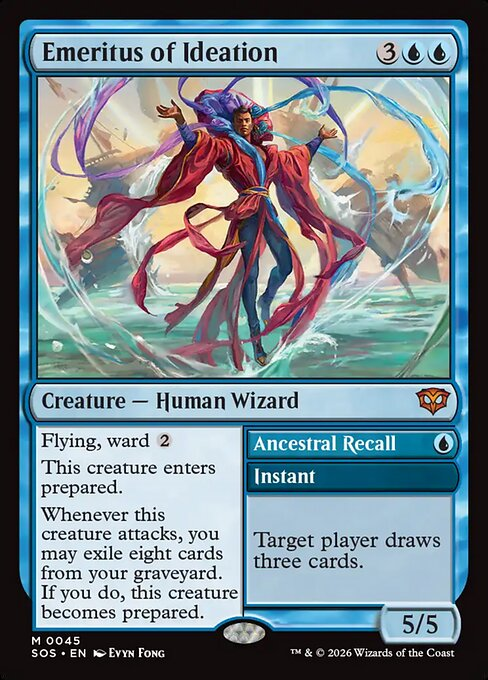
\includegraphics[width=0.24\linewidth]{figures/cards/emeritus-of-ideation.jpg}
\caption{Emeritus of Ideation, an actual first pick from a real thirteen-card
SOS pack (empty pool). The per-set ceiling model (Table~\ref{tab:main})
ranks it above every other card in the pack by a wide margin: real
expected value\protect\footnotemark{} \VHeroEv, seen in \VHeroGih{} of games it's
in, average last-seen-at pick \VHeroAlsa, and \VHeroDominance{} model
dominance over the closest candidate in the pack (\VHeroRunnerOneName).
SOS is a public development set, never the frozen MSH test set
(\S\ref{sec:protocol}); this figure illustrates the model's output, not a
headline result. Numbers regenerated by
\texttt{figures/make\_verdict\_panels.py}.}
\label{fig:teaser}
\end{figure}
\footnotetext{\emph{Expected value} is this per-set model's own raw score
for the card (higher is better; not a model input, and not the top-1
agreement metric reported elsewhere in this paper). \emph{GIH\%} and
\emph{ALSA} are \seventeenlands{} per-card statistics reported for
context: GIH\% is win rate in games where the card was drawn, and ALSA is
the average pick number at which the card was last seen (lower means
drafters value it more highly). \emph{Model dominance} is this paper's
own pairwise measure, $\mathrm{sigmoid}(\text{top EV} - \text{runner-up
EV})$.}
\FloatBarrier

\section{Related work}
\label{sec:related}

\paragraph{Generalised card representations.}
Bertram, F\"urnkranz, and M\"uller~\citep{bertram2024cards} established the
zero-shot drafting problem, and their paper remains the only published
quantitative result on it. They replace one-hot card identities with
concatenated feature vectors: hand-engineered attributes plus a
Sentence-BERT embedding~\citep{reimers2019sbert} of card text (1306-d), a
learned autoencoding of card images (1024-d), and 16 post-release usage
statistics from \seventeenlands{}. This lives inside a
contextual-preference-ranking model trained with a triplet loss. Two of
their findings shape our design: feature
representations match one-hot accuracy within a set (nothing is lost by
generalising), and multi-set pretraining, not the representation alone, is
what buys transfer. Pretrained on 13 sets and evaluated on held-out BRO,
their best representation reaches 55.44\% pick agreement. That
representation includes the usage-statistics block, which is computed from
human play after a set's release; the number is therefore an anchor for
zero-shot \emph{card generalisation} rather than for day-one deployment,
where such statistics cannot exist. The same paper's day-one-feasible
representation (features only) reaches 33.6--35.6\% on unseen sets under
single-set training. No multi-set features-only number is published.
Filling that gap (multi-set training, public card information only) is
this paper's headline experiment, and we adopt their held-out BRO as a
development set so the comparison is on the same holdout. A companion
paper~\citep{bertram2024infonce} improves the within-set triplet objective
with an adapted InfoNCE loss but reports no unseen-set results.

\paragraph{Within-set pick models.}
Ward et al.~\citep{ward2021drafting} compare heuristic and neural drafters
on M19 and report the two most useful reference points below the
data-driven regime: an expert-tuned rating bot at 44.5\% top-1 agreement
and a random agent at 22\%. Their neural drafter (48.7\%) and its
successors, the statistical-drafting MLPs deployed at
statisticaldrafting.com~\citep{brooks2024statistical} (${\sim}70\%$) and
Czerner's puder transformer~\citep{czerner2025puder} (71\%), define the
within-set state of the art, and the statistical-drafting architecture is
the direct lineage of the per-set ceiling models we compare against.
All are one-hot models over a fixed card vocabulary; none can score an
unseen set. The deployment gap is explicit: statistical-drafting documents
that no model can ship until \seventeenlands{} data appears, roughly two
weeks post-release~\citep{brooks2024statistical}, and Draftsim's day-one
ratings are written by human experts~\citep{draftsimratings}.

\paragraph{LLMs as drafters.}
UrzaGPT~\citep{bertram2025urzagpt} evaluates large language models on draft
picks. Zero-shot GPT-4o reaches 43\%, narrowly above the hour-zero rarity
heuristic we measure (\S\ref{sec:results}). We still mark it non-day-one
in Table~\ref{tab:baselines}: NEO shipped years before GPT-4o's training
cutoff, so its pretraining corpus cannot be shown free of the set's own
post-release strategy discussion, a leak a frozen feature-only encoder
cannot have. Providing full rules text in the prompt lowers GPT-4o's
accuracy further. Open 7--8B models fail to pick legal cards until
LoRA-tuned on a million picks from the target set, after which they still
trail small supervised MLPs at orders of magnitude more inference cost. We
take the implied guidance: use a frozen text \emph{embedding} as one
feature block, not a language model as the policy.

\paragraph{Text-grounded transfer in card games.}
Cardsformer~\citep{xia2023cardsformer} encodes Hearthstone card
descriptions with a language model so a gameplay policy generalises to
unseen cards. It is the closest cross-game precedent for text-mediated
transfer, applied to gameplay rather than drafting.

\section{Data}
\label{sec:data}

\paragraph{Corpus.}
Training data is the complete \seventeenlands{} public draft-data
corpus~\citep{seventeenlands}, spanning every set the model has to
generalise across: 31 expansions from STX (April 2021) through
SOS (June 2026), Premier (best-of-one) and Traditional (best-of-three) draft
where published, 59 (set, format) files, roughly 160M pick rows. Each row is
one human pick: the pack contents, the drafter's pool, the card taken, and
two coarse skill covariates (recent game-count bucket and win-rate bucket).
Files were fetched once from the public S3 bucket, per the
\seventeenlands{} usage guidelines (bulk downloads only), and frozen by
sha256 and ETag in a data manifest (content hash
\texttt{\DataManifestHash}); the manifest is released with the paper.

Three public files are excluded for structural reasons, recorded in the
corpus registry: OM1 (a pick-two format whose rows carry two picks and
whose pool columns undercount them, and whose digital-only cards largely do
not exist on Scryfall), the Powered Cube (a curated 545-card singleton pool
with no expansion structure), and the VOW QuickDraft file (human picks
inside bot pods, off-distribution pack dynamics). Everything else is kept,
including digital-only and remaster sets.

\paragraph{Normalization.}
The corpus spans three schema eras and several quirks, all normalised at
ETL time: the 2021 files are gzipped tarballs rather than plain gzipped
CSVs, and the oldest era reports match-based rather than game-based skill
buckets (harmonised; identical in best-of-one). Six sets are missing the
first pick of each draft in the source logs (an annotation, not an
exclusion), and packs are 13, 14, or 15 picks depending on the set (a model
input, \S\ref{sec:method}). Card names are joined to Scryfall by
normalised name with an explicit alias table; unresolved names fail the
build rather than featurizing as zeros. Per set we retain every valid pick
and tag it with the drafter's skill covariates: training filters no one
out. Skill is a conditioning input (``decision + tag by venue'').

\paragraph{Splits.}
Within each (set, format) shard, drafts are split by a hash of the draft
identifier (\texttt{crc32 \% 1000 < 50}, ${\sim}5\%$ validation). Early
stopping uses only this within-training-set validation split. The \emph{expert slice} used for all headline evaluation
is picks by drafters with win-rate bucket $\geq 0.55$ and game-count bucket
$\geq 100$, the same filter the per-set ceiling models train and evaluate
on, so ceiling comparisons are population-matched.

\paragraph{The held-out sets.}
Four sets never contribute a pick to training. BRO, TMT, and SOS are the
development trio (\S\ref{sec:protocol}): all model selection keys on
zero-shot accuracy over these three. MSH, the test set, is stricter: a
registry-level gate (\texttt{EVAL\_ONLY}) makes every training and
feature-fitting code path refuse MSH pick data outright, and at the
protocol freeze its public data did not yet exist. MSH \emph{card} features
from Scryfall are permitted. That is the zero-shot
contract: public card information only, no human behavioral data of any
kind.

\section{Method}
\label{sec:method}

\subsection{Cards as frozen feature vectors}
\label{sec:features}

Every card is a fixed 775-dimensional vector computed from public
information alone, frozen before training.

\paragraph{Structured features (391-d).}
Parsed from the card's Scryfall record: mana value (scaled + bucketed
one-hot, 10), mana-cost pips including hybrid/Phyrexian/X structure (10),
colors (8), color identity (5), supertypes (3), card types (9), creature
subtypes (top-128 vocabulary + an unmatched count, 129), power / toughness
/ loyalty each as (scaled, missing, star) triples (9), rarity (5), keyword
abilities (166 slots + unmatched count, 167), layout including back-face
flags for double-faced cards (10), and text-shape features: length, line
count, and 24 regex flags over rules text for common functional categories
(removal, card draw, counterspells, tokens, ramp, \ldots) (26).
Double-faced and split cards take numeric blocks from the front face.
Subtype and keyword vocabularies are counted over \emph{training} sets
only; a registry gate refuses to fit vocabularies on MSH, the frozen test
set (\S\ref{sec:protocol}). That guarantee covers MSH specifically. It does
not mean the dev trio's cards were excluded from every vocabulary in the
release (\S\ref{sec:data}), so calling the dev trio ``zero-shot'' is a
claim about training picks, not about where the vocabulary came from. The
resulting featurizer manifest is content-hashed
(\texttt{\FeaturizerHash}) and released; held-out cards featurize through
the frozen manifest, with out-of-vocabulary subtypes and keywords absorbed
by the unmatched counters. Scalars are clipped to $[0,1]$; parse failures
set a missing indicator, never a silent zero.

\paragraph{Text embedding (384-d).}
The card's type line and rules text, embedded with a frozen
\texttt{bge-small-en-v1.5} sentence encoder~\citep{xiao2023bge}
($L_2$-normalised). The card's own name, and for legendary cards its
short name, is masked to a placeholder token before embedding, so the
encoder cannot key on names it may know from pretraining. This is a
deliberate handicap, and it matters for licensed-IP sets
(\S\ref{sec:analysis}). Parenthetical reminder text is kept, since for a
brand-new mechanic it is the only definition the model will ever see. Back faces are appended for
double-faced cards.

\subsection{Architecture}
\label{sec:arch}

DraftFM is a two-tower scorer with \FdevParams M parameters (Figure~\ref{fig:arch}). Its two design
invariants operationalize the zero-shot contract (\S\ref{sec:data}):

\begin{enumerate}
  \item \textbf{No set identity.} There is no set embedding and no
  per-card parameter anywhere. The only way the model can know what set it
  is drafting is a \emph{set-context tower} that reads the set's full card
  list, plus the drafter's accumulating pool. ``Blue is the aggressive
  color in this set'' must be inferred from the card list, not memorized
  as a set identifier. Whether the tower itself turns out to be necessary
  for that inference, or whether the invariant holds just as well without
  it, is addressed later in this section.
  \item \textbf{Skill conditions the scorer, not the cards.} Card
  semantics are skill-invariant; the pick policy is not. Skill-bucket
  embeddings enter only the context pathway. Serving conditions on a fixed
  high-skill bucket; training sees every pick tagged with its drafter's
  bucket.
\end{enumerate}

\begin{figure}[t]
\centering
% Architecture diagram for the two-tower model (sections/method.tex, S4.2).
% Pure TikZ, no external assets -- compiles standalone as part of main.tex.
% \input from within a figure environment; see sections/method.tex.
\definecolor{archbox}{HTML}{F2F3F5}
\definecolor{archline}{HTML}{5B6472}
\definecolor{archblue}{HTML}{2563B0}
\definecolor{archmuted}{HTML}{6B7280}

\resizebox{\linewidth}{!}{%
\begin{tikzpicture}[
  font=\small,
  node distance=6mm and 8mm,
  archbox/.style={draw=archline, thick, rounded corners=1.5pt, fill=archbox,
              minimum height=8mm, align=center, inner sep=1.8mm},
  archtower/.style={draw=archblue, thick, rounded corners=1.5pt, fill=archblue!8,
              minimum height=9mm, align=center, inner sep=1.8mm},
  archarr/.style={-{Latex[length=2mm]}, thick, draw=archline},
]
  \node[archbox] (feat) {card feature\\vector\\\scriptsize 775-d};
  \node[archbox, right=of feat] (enc) {shared card\\encoder\\\scriptsize LayerNorm$\to$775--512--256, GELU};
  \node[archbox, right=of enc] (emb) {card\\embeddings\\\scriptsize 256-d};

  \node[archtower, above right=9mm and 9mm of emb] (ctx) {set-context tower\\\scriptsize cross-attn + rarity emb};
  \node[archtower, below right=9mm and 9mm of emb] (pool) {pool tower\\\scriptsize cross-attn, 4 queries};

  \node[archbox, above=7mm of ctx] (ctxin) {full set card list\\\scriptsize $\sim$400 rows};
  \node[archbox, below=7mm of pool] (poolin) {drafter's pool\\\scriptsize distinct cards + count emb};

  \node[archbox, right=15mm of ctx, yshift=-9mm] (cmlp) {context MLP\\\scriptsize +skill, format,\\pick-position feats};
  \node[archbox, right=10mm of cmlp] (score) {scorer MLP\\\scriptsize $[c;\,p;\,c{\odot}p;\,\mathrm{ctx}]$};
  \node[archbox, right=9mm of score] (softmax) {softmax\\\scriptsize over pack};

  \draw[archarr] (feat) -- (enc);
  \draw[archarr] (enc) -- (emb);
  \draw[archarr] (emb.north) .. controls +(0.5,0.3) and +(-0.7,0.1) .. (ctx.west);
  \draw[archarr] (emb.south) .. controls +(0.5,-0.3) and +(-0.7,-0.1) .. (pool.west);
  \draw[archarr] (ctxin) -- (ctx);
  \draw[archarr] (poolin) -- (pool);
  \draw[archarr] (ctx.east) -- (cmlp.north -| ctx.east) -- (cmlp.north);
  \draw[archarr] (cmlp) -- (score);
  \draw[archarr] (pool.east) .. controls +(1.0,0) and +(-1.0,-0.6) .. (score.south);
  \draw[archarr] (emb.south) .. controls +(0.4,-2.4) and +(-2.8,-1.7) .. (score.south)
    node[pos=0.24, above, font=\scriptsize, text=archmuted] {candidate $c$};
  \draw[archarr] (score) -- (softmax);
\end{tikzpicture}%
}

\caption{The two-tower scorer (\S\ref{sec:arch}). A shared card encoder
embeds every card once per (set, format) step; a pool tower summarises
the drafter's held cards, a set-context tower summarises the full card
list, and a per-candidate scorer combines the candidate embedding
$c$, the pool summary $p$, their elementwise product, and the context
vector into a softmax over the pack.}
\label{fig:arch}
\end{figure}

A shared \emph{card encoder} (LayerNorm $\to$ 775--512--256 MLP, GELU)
maps feature vectors to $d{=}256$ embeddings. Because training batches are
homogeneous in (set, format), the encoder runs once per step over the
set's full card list ($\sim$400 rows) and everything downstream gathers
rows from that table. The \emph{pool tower} represents the drafter's pool
as the set of distinct cards held, each embedding translated by a learned
count embedding (counts capped at 8), pooled by cross-attention from four
learned queries (4 heads); an empty pool attends over a learned null token.
The \emph{set-context tower} applies the same query-pooling to the entire
card list (with a rarity embedding added) to produce the set summary. A
context MLP combines the set summary with skill and format embeddings,
seven pick-position features (pack/pick indices, pool size), and four
set-shape scalars (card-list size, picks-per-pack indicator) into a 64-d
context. Each candidate $c$ in the pack is scored by an MLP over
$[\,c;\; p;\; c \odot p;\; \mathrm{ctx}\,]$, where $p$ is the pool summary
and $c \odot p$ the elementwise interaction; a softmax over the pack's
real slots gives the pick distribution.

We test the set-context tower's contribution directly with an experiment
that removes it and retrains; we call this variant A-noctx
(Table~\ref{tab:ablations}, \S\ref{sec:analysis}). It scores higher on all
three dev sets. That tower-free configuration, not the one just described,
is what F-full and the frozen MSH evaluation actually run. The first invariant still holds
either way, since neither configuration has a set-identity parameter.
Dropping the tower simply means the shipped model's only route to
set-relative signal is the pool tower, each candidate's own features, and
the four set-shape scalars above; it never reads the rest of the card
list.

\subsection{Training}
\label{sec:training}

One optimization recipe governs every run in the paper. It was fixed before the
scaling and variant studies, since the protocol forbids per-rung tuning.
Batches of 8{,}192 picks are drawn from one (set, format) shard at a
time. Shards are sampled proportionally to $n_{\text{picks}}^{0.5}$, an
interpolation between pick-uniform sampling, which lets the largest sets
dominate, and set-uniform sampling, which oversamples tiny sets. The
optimizer is AdamW ($\beta_1{=}0.9$, $\beta_2{=}0.98$, weight decay 0.01)
with peak learning rate $10^{-3}$, a 2{,}000-step linear warmup, and
cosine decay; the loss is cross-entropy with label smoothing 0.05,
renormalised over real pack slots. The presentation budget
is four epochs. Within-training validation (never the dev sets) is
evaluated every 2{,}000 steps and training stops after three
non-improving evaluations. Seed 17 throughout. Seed variance is measured
at two scaling rungs (\S\ref{sec:protocol}).

Training runs on a single Apple M3 Ultra workstation (96\,GB unified
memory) in PyTorch 2.12 eager mode on the MPS backend, at
$\sim$\FdevExamplesPerSec{} picks/s. The full \FdevPicks M-pick run takes
about \FdevWallHours{} hours, stopping at step 34{,}000. Training-backend
correctness is gated rather than assumed; specifics are in the companion
reference. Inference exports to ONNX (opset 18) and runs on a consumer
x86-64 machine, CPU-only, well under a millisecond per pick.

\section{Pre-registered evaluation protocol}
\label{sec:protocol}

The substantive evaluation design was frozen at the public git tag
\texttt{eval-protocol-v1} on July 4, before MSH pick data was public. The
single evaluation ran under \texttt{\ProtocolTag}, a hardening tag cut on
July 7 after an automated downloader had fetched the first snapshot but
before any frozen-battery inference. That tag adds the exact battery
manifest, git-history and feature-manifest guards, and corrections to the
pre-written claims-band boundaries. The full chronology, including a
separate serving pipeline that read the snapshot before the frozen pass,
is disclosed in \S\ref{sec:msh}.

Model weights are too large to version directly, so each battery member's
weights are anchored by the sha256 recorded in the tagged manifest. The
enforcer cross-checks the experiment ledger's git history to confirm that
every battery weight was committed before the first MSH download, and a
hash guard refuses to run if the metric code has drifted from
\texttt{\ProtocolTag}. There is one evaluation round; a second round would
require a new public tag and disclosure that a second round happened. One
terminological note for auditors: the tagged protocol uses the name
``expert slice'' for the population this paper calls high-win-rate players
(\S\ref{sec:data}); the filter is identical, so the two terms map one to
one.

\subsection{Test set: MSH, exactly once}

MSH is the first \mtg{} set drafted on Arena after the protocol freeze. It
is a licensed-IP (\emph{Universes Beyond}) set, which makes the test
deliberately harder (\S\ref{sec:analysis}). The protocol defines the test
snapshot as the first public \seventeenlands{} MSH Premier file
successfully downloaded on or after its publication, frozen immediately by
sha256 and ETag and never re-downloaded. Until the frozen evaluation has
run, no training, tuning, metric-peeking, or feature-vocabulary fitting
may read MSH pick data. MSH \emph{card} features alone are legal, per the
zero-shot contract of \S\ref{sec:data}. The snapshot must pass quality
gates: modern schema, Premier rows present, at least 2{,}500 drafts from
the high-win-rate slice, and $\geq 99\%$ of pack card names joining to
card features. On a volume failure the single pre-declared contingency is
to wait exactly one snapshot cycle. The evaluation must execute within 72
hours of the gates passing: one inference pass per battery member over the
frozen snapshot, cached as per-pick prediction files from which every
statistic is computed. Models are never re-run during analysis. The
execution of this protocol, and its outcome, are reported in
\S\ref{sec:msh}.

Two populations are scored. The high-win-rate slice (\S\ref{sec:data}) is
the headline; the all-users slice is secondary. Two conditioning
configurations are pre-registered. \emph{Deployment mode}, the headline,
conditions on a fixed top skill bucket selected on the dev sets and frozen
into the battery configuration. \emph{Human-model mode} conditions on each
drafter's true bucket and is scored on all users. Forced picks, the final
pick of a pack, are included in headline numbers, matching the within-set
references and prior work; non-forced variants are secondary rows.

\subsection{Development discipline}

One number governs every architecture, hyperparameter, text-encoder, and
conditioning decision in this paper: mean top-1 agreement, on the
high-win-rate slice in deployment mode, averaged unweighted over three
sets (BRO, TMT, SOS), with ties broken by mean log-loss. That number comes
from a single development run, \emph{F-dev}, trained on every set except
those three and MSH.

We chose that trio for three separate reasons. BRO is the same holdout used
by the only published multi-set, feature-based zero-shot
number~\citep{bertram2024cards}, so it supplies a same-set reference; the
different pick populations and information regimes are disclosed with the
result. SOS is the set where our own per-set model is most mature, giving
the strongest available within-set reference. And TMT is a
licensed-IP set, so it rehearses the same distribution shift MSH will
present. Early stopping never looks at these dev metrics
(\S\ref{sec:training}), so the curve reported later in \S\ref{sec:results}
is not selected on the same axis it is plotted against.

\subsection{Metrics and statistics}

The primary metric is top-1 agreement with the human pick, on the
high-win-rate slice in deployment mode. Several secondary metrics
accompany it: top-3 agreement; all-users top-1 in human-model mode; the
\emph{normalized score}, which divides the model's zero-shot top-1 by the
top-1 of a supervised reference trained directly on the target set and
aligned pick-by-pick on its validation split; mean log-loss; top-label
expected calibration error,
computed over 15 equal-mass bins with a temperature fit on the dev trio
only, frozen into the battery before T0, and never fit on the test set
itself (\S\ref{sec:analysis}); per-(pack, pick) accuracy curves against
the per-cell random floor; and \emph{late-draft retention}, the same
zero-shot-to-reference ratio restricted to picks 8 and later of each pack,
where pool context dominates.

All intervals are cluster bootstraps over drafts, not picks
($B{=}2{,}000$, fixed seed, percentile 95\% CIs); paired comparisons share
resample indices. Clustering matters little, but the choice is grounded
empirically. The measured intraclass correlation of pick correctness
within drafts is $\rho = 0.0099$ (per-set SOS validation; 1{,}662 drafts,
69{,}803 picks), a design effect of ${\sim}1.4$ at ${\sim}42$ picks per
draft. That gives CI half-widths of about $\pm0.36$pp at the
2{,}500-draft gate, under a binomial approximation at $p{=}0.5$. Seed
variance is measured with three seeds at two scaling rungs, and
set-composition variance with two probe rungs (\S\ref{sec:results}).

\subsection{The battery}

Frozen by artifact hash before the test snapshot:
(1)~\textbf{F-full}, the final recipe trained on all 31 sets, the headline
model; its dev-set numbers are meaningless (it trains on them) and are
never quoted. A pre-registered flexibility clause lets two optional extras
(the Powered Cube file and VOW QuickDraft) join F-full's training data if
and only if a dev-trio comparison shows a gain; the decision is frozen
with the battery and reported either way.
(2)~\textbf{F-dev}, the development model described above, which doubles
as the top scaling rung.
(3)~\textbf{Scaling rungs} at 1, 2, 4, 8, 16, and 28 training sets
(nested, in release order) plus two composition probes, all with the fixed
recipe and a shared step cap.
(4)~\textbf{Variants}: A-notext, which removes the text embedding and
keeps structured features only, and A-noUB, which removes the three
licensed-IP training sets, both for the shift analysis of
\S\ref{sec:analysis}.
(5)~\textbf{Baselines}: random; an hour-zero rarity-color heuristic; and
three asterisked post-release baselines (community site ratings at
day~$\sim$2, and two \seventeenlands{}-statistics pickers) that bound what
cheap post-release information buys.
(6)~\textbf{Post-day-one rows}, frozen now and executed only after the
zero-shot evaluation: a within-set supervised reference trained on the frozen MSH snapshot
with the stock per-set recipe, and F-full fine-tuned on the MSH training
split with hyperparameters pinned from dev-trio trial runs.

\subsection{Claims bands}

To keep interpretation out of our own hands, three mutually exclusive
claims paragraphs (for headline results below 45\%, between 45 and 55\%,
and above 55\%) were drafted before any test number existed and are
carried in the paper source; the matching one is selected verbatim when
the frozen evaluation reports (\S\ref{sec:msh}). In all bands the
secondary claims are the same: relative agreement to the within-set reference, the shape
of the scaling curve, the analysis of what the text embedding contributes
under the licensed-IP shift, and the skill-conditioning effect.

\section{Results on the development sets}
\label{sec:results}
\FloatBarrier

\begin{table}[t]
  \centering
  \caption{Zero-shot top-1 agreement (\%) with high-win-rate players,
  deployment mode, forced picks included; 95\% cluster-bootstrap
  confidence intervals over drafts in parentheses. Sets: The Brothers'
  War (BRO), Teenage Mutant Ninja Turtles (TMT), Secrets of Strixhaven
  (SOS), and Marvel Super Heroes (MSH). F-full's dev-trio cells are never
  quoted, since it trains on those three sets.}
  \label{tab:main}
  \footnotesize
  \setlength{\tabcolsep}{2.4pt}
  % The CI columns make this a hair wider than \textwidth; center the
  % overhang symmetrically instead of letting it spill into one margin.
  \makebox[\textwidth][c]{% AUTO-GENERATED by scripts/make_paper_tables.py -- do not edit.
% Main results: expert-slice deployment-mode top-1 (95% cluster-bootstrap CIs over drafts).
\begin{tabular}{lccccc}
\toprule
Model & BRO & TMT & SOS & Dev mean & MSH \\
\midrule
DraftFM (F-dev, zero-shot) & 48.9 {\scriptsize(48.8, 49.0)} & 57.5 {\scriptsize(57.3, 57.7)} & 56.5 {\scriptsize(56.4, 56.6)} & 54.3 & \pendingcell \\  % run=20260704_135822_f_dev; run=20260704_135822_f_dev; run=20260704_135822_f_dev; run=20260704_135822_f_dev; pending: eval
DraftFM (F-full, zero-shot) & -- & -- & -- & -- & \pendingcell \\  % pending: eval
\midrule
Per-set ceiling & 65.6 & 71.0 & 70.2 {\scriptsize(69.8, 70.6)} & 68.9 & \pendingcell \\  % run=perset-BRO-latest; run=perset-TMT-latest; run=perset-SOS-protocol-validation; pending: post-T0
\quad F-dev / ceiling (unaligned) & 0.745 & 0.810 & 0.805 & 0.787 & \pendingcell \\  % pending: post-T0
\bottomrule
\end{tabular}
}
\end{table}

\paragraph{Zero-shot transfer on the development trio.}
% Aligned normalized score (scripts/eval_normalized_score.py, inner-joined
% on identical (draft_id, pack, pick) so zero-shot and ceiling score the
% same picks -- a much smaller aligned subset than the unaligned ratio's
% full slice, since the ceiling model's val split is small): run=
% 20260704_135822_f_dev. BRO 0.7430 (CI 0.7363-0.7503, n=59,572 aligned
% picks), TMT 0.8132 (CI 0.8015-0.8251, n=17,261), SOS 0.8019 (CI
% 0.7960-0.8077, n=69,803), dev-mean 0.7860.
Table~\ref{tab:main} reports zero-shot transfer on the development trio.
F-dev, the recipe used for architecture and hyperparameter selection,
trains on \FdevPicks M picks from \FdevSets{} sets and is then evaluated
on three sets it has never seen a pick from, where it agrees with
high-win-rate players on \FdevDevMean\% of picks. Every number in this
paragraph is a dev-trio rehearsal by the protocol's own design; the
paper's headline is the frozen MSH result of \S\ref{sec:msh}. Broken out
per set, DraftFM reaches \FdevBro\% / \FdevTmt\% / \FdevSos\% on BRO /
TMT / SOS. For comparison, a model trained directly on each of those
sets, the ceiling, reaches \CeilBro\% / \CeilTmt\% / \CeilSos\%.
DraftFM's pre-registered normalized score, its accuracy as a fraction of
that ceiling on identical held-out picks per \S\ref{sec:protocol}, is
\NormScoreBro\% / \NormScoreTmt\% / \NormScoreSos\%, with dev-mean
\NormScoreDevMean\%. A simpler, unaligned version of the same ratio,
taken over the full slice rather than the smaller aligned subset,
corroborates this on a much larger sample: \RatioBro\% / \RatioTmt\% /
\RatioSos\%, dev-mean \RatioDevMean\%. That unaligned ratio is not
itself the pre-registered metric, since the aligned version is capped by
the size of the ceiling model's own held-out split. Excluding forced
picks lowers the three numbers to \FdevBroNonForced\% /
\FdevTmtNonForced\% / \FdevSosNonForced\%. The deployment-mode skill
bucket selected on dev is the \DeployBucket{} win-rate bucket.

\paragraph{Reading the BRO row.}
BRO is the holdout on which \citet{bertram2024cards} report 55.4\%, the
strongest published unseen-set number. They reach it with card features,
learned image embeddings, and 16 usage statistics computed from human
play after the set's release, scored on all players rather than a
win-rate-filtered population. Our \FdevBro\% on the high-win-rate slice,
\FdevBroAllUsers\% on all players as the population-matched comparator,
is below that number, but the two are not a fair fight: their number
assumes information that does not exist on release day. The fair
comparison is against what the same paper achieves without post-release
usage statistics, 33.6--35.6\% on a single set, and every other
day-one-feasible baseline in Table~\ref{tab:baselines}. Against that
day-one bar, multi-set training on public card features closes most of
the distance to the usage-statistics number while using only release-day
information.

BRO is also the hardest set in the trio for transfer: its packs mix in a
63-card retro-artifact bonus sheet, examined directly in
\S\ref{sec:analysis}. Why TMT, the trio's licensed-IP set, nonetheless
transfers as well as SOS, and why BRO lags both, is analysed there too.
Figure~\ref{fig:tmt-tierlist} shows a real P1P1 bomb from TMT scored the
same way. For sets that are in the training corpus but have no dedicated
per-set model, the deployed system falls back to F-full's scoring;
Figure~\ref{fig:gallery} shows what that fallback looks like today for
LTR, LCI, and DMU.

\begin{figure}[t]
\centering
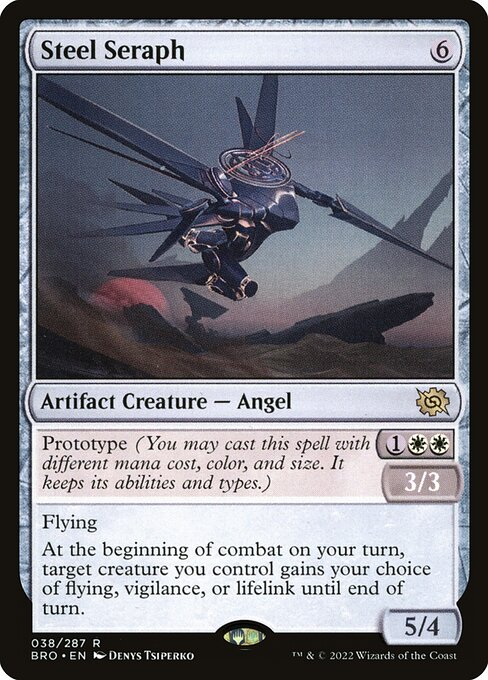
\includegraphics[width=0.24\linewidth]{figures/cards/steel-seraph.jpg}
\caption{Steel Seraph, BRO, the dev trio's hardest transfer set
(\S\ref{sec:analysis}). Real P1P1 expected value \VBroEv, the
\VBroPercentile{}th percentile of BRO's card pool by the deployed per-set
model's own ranking; the next two candidates in the pack,
\VBroRunnerOneName{} and \VBroRunnerTwoName{}, rank at the
\VBroRunnerOnePercentile{}th and \VBroRunnerTwoPercentile{}th. Percentile,
not a head-to-head split: Arena hides the pack between picks in this mode
(\S\ref{sec:arch}).}
\label{fig:bro-tierlist}
\end{figure}

\begin{figure}[t]
\centering
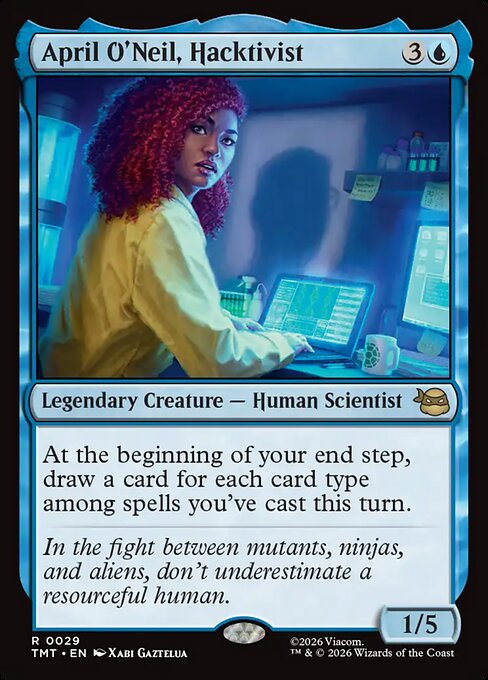
\includegraphics[width=0.24\linewidth]{figures/cards/april-oneil-hacktivist.jpg}
\caption{April O'Neil, Hacktivist, TMT, the dev trio's licensed-IP set
(\S\ref{sec:analysis}), a comic-book bomb the text encoder never saw
described in \mtg{} rules-text style. Real P1P1 expected value \VTmtEv,
the \VTmtPercentile{}th percentile of TMT's card pool.}
\label{fig:tmt-tierlist}
\end{figure}

\begin{figure}[t]
\centering
\begin{minipage}[b]{0.20\linewidth}
  \centering
  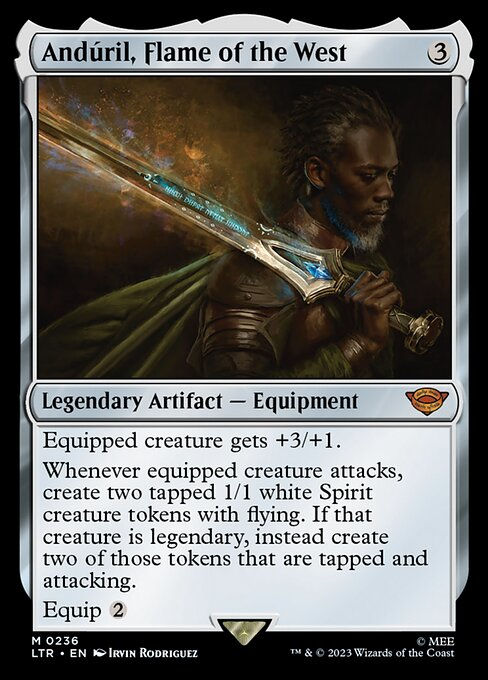
\includegraphics[width=\linewidth]{figures/cards/anduril-flame-of-the-west.jpg}\par
  \small LTR: EV \VGalLtrEv, pct \VGalLtrPercentile
\end{minipage}%
\hfill
\begin{minipage}[b]{0.20\linewidth}
  \centering
  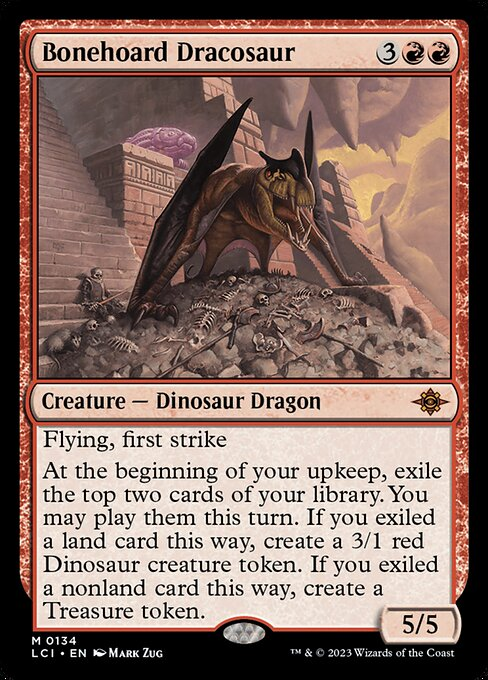
\includegraphics[width=\linewidth]{figures/cards/bonehoard-dracosaur.jpg}\par
  \small LCI: EV \VGalLciEv, pct \VGalLciPercentile
\end{minipage}%
\hfill
\begin{minipage}[b]{0.20\linewidth}
  \centering
  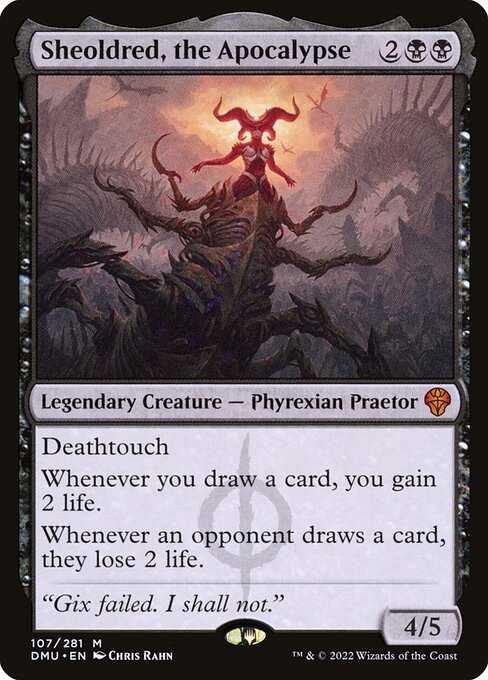
\includegraphics[width=\linewidth]{figures/cards/sheoldred-the-apocalypse.jpg}\par
  \small DMU: EV \VGalDmuEv, pct \VGalDmuPercentile
\end{minipage}
\caption{Three sets with no dedicated per-set model: The Lord of the
Rings: Tales of Middle-earth (LTR), The Lost Caverns of Ixalan (LCI),
and Dominaria United (DMU), all in F-full's 31-set training corpus.
Expected values and percentiles are computed as in
Figures~\ref{fig:bro-tierlist} and \ref{fig:tmt-tierlist}. Because
F-full trained on these three sets, the figure shows the deployed
fallback path a newly released set would use before a per-set model
exists for it; it is not a zero-shot accuracy claim.}
\label{fig:gallery}
\end{figure}

\begin{table}[t]
  \centering
  \caption{Measured baselines: top-1 agreement (\%) with high-win-rate
  players, deployment mode. Rows marked $^{*}$ use post-release
  information and bound what cheap human data buys within days of a
  set's release. Published numbers from prior work, which differ in test
  set, information regime, and pick population, appear in
  Table~\ref{tab:prior-work}.}
  \label{tab:baselines}
  \footnotesize
  \setlength{\tabcolsep}{3.5pt}
  % AUTO-GENERATED by scripts/make_paper_tables.py -- do not edit.
% Measured baselines (hour-0 and asterisked post-release). Published prior numbers are in prior_work.tex.
\begin{tabular}{llll}
\toprule
\rowcolor{tblhead}
Method & Information used & Test set & Top-1 agreement (\%) \\
\midrule
Random & none & MSH & 23.3 {\scriptsize(23.1, 23.4)} \\  % run=frozen_eval/013df16b8994
Rarity--color heuristic & card features (hour 0) & MSH & 25.6 {\scriptsize(25.4, 25.7)} \\  % run=frozen_eval/013df16b8994
Site-ratings heuristic (day $\sim$2)$^{*}$ & post-release statistics & MSH & \pendingcell \\  % pending: post-T0
ALSA-argmin$^{*}$ & post-release statistics & MSH & \pendingcell \\  % pending: post-T0
shrunk-GIH-argmax$^{*}$ & post-release statistics & MSH & \pendingcell \\  % pending: post-T0
\bottomrule
\end{tabular}

\end{table}

\paragraph{Baselines.}
Table~\ref{tab:baselines} reports the baselines we measure ourselves;
published numbers from prior work are situated in
Table~\ref{tab:prior-work} in the introduction. The table's rows are
scored on the frozen MSH snapshot; before the freeze, the same two
hour-zero baselines were rehearsed on SOS, where random picking scored
\BaseRandom\% and a heuristic that prefers lower rarity for playables
and follows the pool's colors reached \BaseRarity\%. That rehearsal
figure lands just below GPT-4o's 43\% \citep{bertram2025urzagpt} and
close to the expert-tuned 44.5\% of \citet{ward2021drafting}, a useful
caution about how much of drafting, on an in-universe set, is surface
regularity. The same heuristic does far worse on MSH itself
(\BaseRarityMsh\%, discussed in \S\ref{sec:msh}), so that caution cuts
both ways. DraftFM's zero-shot numbers clear every day-one-feasible
baseline on each of the three dev sets. The three asterisked
post-release baseline rows remain pending; their recipes were never
frozen before the snapshot arrived, and \S\ref{sec:msh} explains why we
leave them open rather than define them after the fact.

\begin{figure}[t]
  \centering
  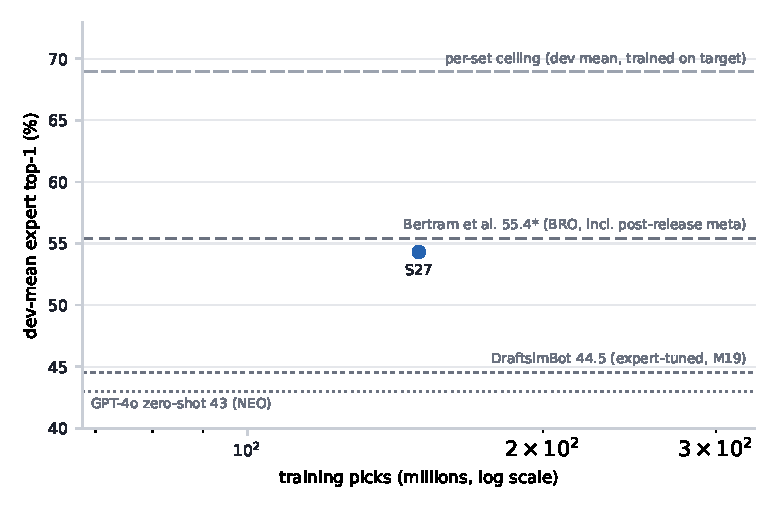
\includegraphics[width=0.78\linewidth]{figures/scaling_curve.pdf}
  \caption{Zero-shot dev-trio-mean top-1 agreement with high-win-rate
  players vs.\ training picks (log scale). Filled points: the nested
  scaling ladder; open points: set-composition probes. Horizontal rules
  mark published anchors and the per-set ceiling mean.}
  \label{fig:scaling}
\end{figure}

\begin{table}[t]
  \centering
  \caption{Scaling ladder. Rung labels are frozen protocol identifiers, not
  set counts: \emph{S27} names the top rung's run, which actually trains on
  28 sets, a naming artifact from an earlier corpus size, kept as-is rather
  than renamed after the fact. Set and pick counts in the table are the
  real values from run records. Dev-mean is the model-selection metric of
  \S\ref{sec:protocol}.}
  \label{tab:scaling}
  \small
  \setlength{\tabcolsep}{4pt}
  % AUTO-GENERATED by scripts/make_paper_tables.py -- do not edit.
% Scaling ladder (protocol section 4.3). Rung labels are frozen identifiers; counts come from run records.
\begin{tabular}{l p{4.8cm} rrrc}
\toprule
\rowcolor{tblhead}
Rung & Sets & \#sets & Train picks (M) & Best step & Dev-mean top-1 (\%) \\
\midrule
S1 & NEO & 1 & 5.4 & 4000 & 48.9 \\  % run=20260704_154741_s1; run=20260704_154741_s1
S2 & S1 + DSK & 2 & 13.3 & 18000 & 50.9 \\  % run=20260704_161450_s2; run=20260704_161450_s2
S2b & MOM, TDM (probe) & 2 & 14.5 & 8000 & 50.2 \\  % run=20260704_171827_s2b; run=20260704_171827_s2b
S4 & S2 + DMU, FIN & 4 & 27.8 & 24000 & 51.7 \\  % run=20260704_175554_s4; run=20260704_175554_s4
S4b & STX, SNC, OTJ, TLA (probe) & 4 & 23.5 & 20000 & 51.0 \\  % run=20260704_191659_s4b; run=20260704_191659_s4b
S8 & S4 + STX, MOM, BLB, TLA & 8 & 52.9 & 18000 & 52.4 \\  % run=20260704_202620_s8; run=20260704_202620_s8
S16 & S8 + AFR, SNC, ONE, LTR, WOE, MKM, OTJ, EOE & 16 & 99.9 & 34000 & 53.3 \\  % run=20260704_213310_s16; run=20260704_213310_s16
S27 & full F-dev universe & 28 & 149.4 & 34000 & 54.3 \\  % run=20260704_135822_f_dev; run=20260704_135822_f_dev
\bottomrule
\end{tabular}

\end{table}

\paragraph{Scaling.}
Figure~\ref{fig:scaling} and Table~\ref{tab:scaling} report zero-shot
accuracy as training grows from one set (NEO, 5.4M picks) to the full
\FdevSets-set universe (\FdevPicks M picks), under the fixed recipe.
Single-set training is the regime of \citet{bertram2024cards}'s
features-only anchor; the top rung is F-dev.
% Seed spread (within-training top-1, not a dev-trio zero-shot re-eval):
% run=20260704_154741_s1 (0.6824), run=20260705_170754_s1_seed18 (0.6774),
% run=20260705_170754_s1_seed19 (0.6768); run=20260704_175554_s4 (0.6892),
% run=20260705_170755_s4_seed18 (0.6881), run=20260705_170755_s4_seed19 (0.6880).
Two extra seeds at S1 and S4 give within-training top-1 spreads of
0.677--0.682 and 0.688--0.689. Training itself is not noise-dominated at
either rung; this checks in-distribution training stability and
complements the zero-shot dev-mean seed spread reported below.
% TODO-DRIVER: the literal seed-spread and composition-probe numbers in
% this paragraph and the next two (0.677-0.682, 0.688-0.689, 50.2, 50.9,
% 51.0, 51.7, pick counts) predate the macros-only rule; macro-ify if
% convenient. Values unchanged here.
% Log-linear fit of dev-mean top-1 on log2(train picks), nested ladder only
% (S1..F-dev/S27): scripts/analyze_scaling_shape.py, reading
% paper/figures/scaling_data.json (same source scaling_curve.py plots from).
% slope=1.037pp/doubling, R^2=0.980, max |residual|=0.43pp (S2). Per-segment
% doubling-normalized deltas: S1-S2 1.57, S2-S4 0.67, S4-S8 0.79, S8-S16
% 1.01, S16-F-dev 1.68 pp/doubling -- non-monotonic, no decay toward the
% top rung.
A log-linear fit of dev-mean top-1 on $\log_2$(training picks) across the
nested ladder (S1 through F-dev, 5.4M--149.4M picks) tracks the six rungs
closely: slope 1.0 percentage point per doubling, $R^2=0.98$, with no rung
off the fitted line by more than 0.4pp. But that same fit argues against
reading a diminishing-returns point into the tested range, not for one.
The per-doubling gain moves between 0.7 and 1.7pp/doubling, and it does so
non-monotonically: lowest across the S2--S8 middle of the ladder, highest
at the S1--S2 start and the S16--F-dev end, rather than decaying toward
the top rung.

Six error-bar-free points, on a fit whose own top rung is the model
selected on this axis, are not strong evidence of log-linearity. The
honest reading is narrower than it looks: no diminishing returns are
visible over the two orders of magnitude tested, which is not the same as
showing that returns do not saturate beyond that range.

Re-scoring those same extra-seed checkpoints on the zero-shot dev-mean the
curve actually plots, rather than on within-training top-1, gives
per-seed spreads of \SeedSpreadSone pp at S1 and \SeedSpreadSfour pp at
S4. That is at most about a quarter of the \SeedGainSoneSfour pp gain from
S1 to S4, so the rung-to-rung climb is not a seed artifact. These are
three-seed spreads at two rungs that also fold in an early-stop-step
difference (the two added seeds stopped at half the reference seed's
step), so they bound the curve's seed noise rather than fully characterize
it, standing in at S1/S4 as a proxy for the top rung.

The two composition probes offer a natural check on whether pick count
alone predicts a rung's score, or whether which sets are in it matters too.
At matched set count, S2b (MOM and TDM, 14.5M picks) scores 50.2\% against
S2's 50.9\%, despite having \emph{more} training picks than S2's 13.3M
(Table~\ref{tab:scaling}). If pick count were the whole story, S2b should
have scored higher, not lower. S4b (23.5M picks) scores 51.0\% against
S4's 51.7\%, in the direction pick count would predict, but S4 also has
more picks (27.8M), so that pair does not separate the two explanations.
Only S2 vs.\ S2b isolates set count from pick count, and on that one pair,
composition beats volume: which sets a rung trains on moves the score more
than how many picks they contribute. Two probe pairs is not enough to
generalize beyond that.

\section{Analysis}
\label{sec:analysis}
\FloatBarrier

\begin{table}[t]
  \centering
  \caption{The variant grid: zero-shot top-1 (\%) with high-win-rate
  players, point estimates (per-cell 95\% CI half-widths are
  ${\sim}\pm0.1$--$0.2$pp on the dev sets, Table~\ref{tab:main};
  paired-difference CIs accompany the deltas in the text). A-noctx,
  A-proportional, and A-topfilter are architecture variants tested
  against the Full baseline before the deployed architecture was fixed.
  A-notext and A-noUB are the two pre-registered comparisons
  (\S\ref{sec:protocol}) analysed below: A-notext drops the 384-d text
  embedding from the Full recipe, and A-noUB removes the three
  licensed-IP training sets from A-noctx (the winning architecture,
  \S\ref{sec:arch}), so its clean comparator is the A-noctx row, not
  Full. The (variant $\times$ set) grid supplies the dev-side measurement
  of what the text embedding contributes on licensed-universe sets
  (per-set deltas below), computed before MSH is seen.}
  \label{tab:ablations}
  \small
  % AUTO-GENERATED by scripts/make_paper_tables.py -- do not edit.
% Pre-registered ablations (protocol section 5).
\begin{tabular}{lccccc}
\toprule
Variant & BRO & TMT & SOS & Dev mean & MSH \\
\midrule
Full (F-dev recipe) & 48.9 & 57.5 & 56.5 & 54.3 & \pendingcell \\  % run=20260704_135822_f_dev; run=20260704_135822_f_dev; run=20260704_135822_f_dev; run=20260704_135822_f_dev; pending: eval
A-notext & \pendingcell & \pendingcell & \pendingcell & \pendingcell & \pendingcell \\  % pending: BRO; pending: TMT; pending: SOS; pending: mean; pending: eval
A-noUB & \pendingcell & \pendingcell & \pendingcell & \pendingcell & \pendingcell \\  % pending: BRO; pending: TMT; pending: SOS; pending: mean; pending: eval
\bottomrule
\end{tabular}

\end{table}

\paragraph{Seed variance on the top-scoring variant.}
% Within-training top-1, not a dev-trio zero-shot re-eval: run=20260704_160422_a_noctx
% (0.6842), run=20260705_110803_noctx_seed18 (0.6803), run=20260705_133440_noctx_seed19
% (0.6796).
Two additional seeds of A-noctx (the recipe F-full uses, \S\ref{sec:arch})
land within-training top-1 at 0.680--0.684, a 0.5pp spread around the seed
reported in the table. So A-noctx's own accuracy is not a single lucky
initialization. But the margins between it and the neighboring
recipe-search variants are close (54.2--54.8 dev-mean,
Table~\ref{tab:ablations}), meaning the full ranking among variants has
not itself been seed-checked.

\paragraph{The flexibility-clause extras.} % run=20260705_220253_a_extras:
% BRO 0.4888 (CI 0.4878-0.4898), TMT 0.5758 (CI 0.5739-0.5776), SOS 0.5601
% (CI 0.5592-0.5611), dev-mean 0.5416, vs. A-noctx's 50.0/57.7/56.6/54.8.
% Paired-difference CIs (scripts/eval_ablation_deltas.py, evalproto.paired_
% bootstrap_diff, shared draft resamples, a_extras - a_noctx): BRO -0.0113
% (CI -0.0120,-0.0107), TMT -0.0015 (CI -0.0026,-0.0003), SOS -0.0057
% (CI -0.0062,-0.0052) -- all three exclude 0, so all three per-set deltas
% are real, not just the BRO one.
The protocol's flexibility clause (\S\ref{sec:protocol}) admits VOW
QuickDraft and the Powered Cube into F-full's training data only if a
dev-trio experiment shows a gain over A-noctx. Adding VOW QuickDraft to
A-noctx (same recipe and holdout, one shard added) scores 48.9/57.6/56.0,
dev-mean 54.2. That is lower than A-noctx's
\ANoctxBro/\ANoctxTmt/\ANoctxSos/\ANoctxDevMean{} on all three dev sets,
and the paired-difference CI excludes zero on every set ($-$1.1pp BRO, CI
$-$1.2 to $-$1.1; $-$0.1pp TMT, CI $-$0.26 to $-$0.03; $-$0.6pp SOS, CI
$-$0.62 to $-$0.52). So the clause's own rule excludes it: F-full's frozen
recipe (\S\ref{sec:arch}) does not train on VOW QuickDraft. The Powered
Cube half of the clause was not tested at all, since bulk per-pick data
for it is not available through the public \seventeenlands{} pipeline this
paper otherwise relies on exclusively, and acquiring it by another route
was out of scope. Both extras are therefore absent from F-full's training
data, one by a pre-registered result that failed to show a gain and the
other by an unmet data precondition, and the frozen recipe is exactly the
31-set corpus described in \S\ref{sec:data}.

\paragraph{What the text embedding contributes on licensed universes.}
MSH's names and flavor come from a comic universe, not from \mtg{}. Its
text lives in the sentence encoder's pretraining as a different genre.
This is the distribution shift most likely to break a text-dependent
model on the day it matters, which is why the protocol makes a
licensed-IP set (TMT) a development set: the rehearsal happens where it
can still inform design. One mitigation is built in: card names are
masked out of the text before embedding (\S\ref{sec:features}), so the
encoder sees mechanics, not franchises. A second design choice does not
reduce the shift but makes it measurable. The comparison grid of
Table~\ref{tab:ablations} separates what the text embedding contributes
on in-universe sets, SOS and BRO, from what it contributes on licensed
sets, TMT and MSH.

Zero-shot, the licensed dev set turns out not to be the hard one. TMT
reaches \FdevTmt\% against SOS's \FdevSos\% (and \RatioTmt\% vs
\RatioSos\% of their respective supervised references), which is
consistent with structured features carrying much of the load. The study
has no unmasked-text control, so it does not isolate name masking's effect.
The pattern could mean text adds little on licensed sets, or it could just
mean TMT is an easier format. The ablations provide association checks,
not a clean separation of those explanations:
% Arithmetic on Table~\ref{tab:ablations}'s own cells, both already
% run-tagged there: A-notext vs. Full (its comparator): BRO 48.9-45.8=3.1pp,
% TMT 57.5-55.9=1.6pp, SOS 56.5-53.1=3.4pp. A-noUB vs. A-noctx (its
% comparator per the table caption, not Full): BRO 50.0-49.2=0.8pp,
% TMT 57.7-57.5=0.2pp, SOS 56.6-54.9=1.7pp.
% Paired-difference CIs (scripts/eval_ablation_deltas.py,
% evalproto.paired_bootstrap_diff, shared draft resamples): text-penalty
% (Full - A-notext): BRO +0.0312 (CI 0.0304,0.0320), TMT +0.0159
% (CI 0.0146,0.0173), SOS +0.0342 (CI 0.0335,0.0349), dev-mean +0.0271.
% UB-penalty (A-noctx - A-noUB): BRO +0.0079 (CI 0.0072,0.0086), TMT
% +0.0021 (CI 0.0009,0.0033), SOS +0.0168 (CI 0.0162,0.0175), dev-mean
% +0.0089. All six per-set deltas exclude 0, including TMT's small 0.2pp
% UB-penalty (CI 0.09-0.33pp) -- pairing on identical held-out picks
% cancels enough between-draft variance that even this small a gap is
% distinguishable from noise, not just directionally suggestive.
dropping text costs TMT only \TextPenTmt pp (CI \TextPenTmtCi pp) against
its Full comparator, less than BRO's \TextPenBro pp (CI \TextPenBroCi pp)
or SOS's \TextPenSos pp (CI \TextPenSosCi pp). Text contributes least on
the sole licensed-IP development set, but that does not identify why.
Removing the three licensed-IP training sets from A-noctx changes BRO by
\UbPenBro pp (CI \UbPenBroCi pp), TMT by \UbPenTmt pp (CI \UbPenTmtCi pp),
and SOS by \UbPenSos pp (CI \UbPenSosCi pp). These paired differences are
statistically distinguishable from zero, but the ablation simultaneously
removes training volume, mechanics, and set composition. It therefore does
not identify a causal benefit of licensed-IP training. With one licensed
development set, the defensible conclusion is only that TMT did not expose
a transfer failure before the frozen MSH test.

\paragraph{Why BRO transfers worst.}
% scripts/eval_bro_transfer_analysis.py, run=20260704_135822_f_dev.
% Headline: BRO 0.4889, mean(TMT,SOS) 0.5701, gap 0.0812 (8.1pp).
% Bonus-sheet slice (BRR 63-card retro-artifact sheet, packs offering >=1
% bonus-sheet card vs. not): bonus_present top1 0.4062 (CI 0.4048-0.4077,
% n=510,654, 44.3% of picks), bonus_absent 0.5547 (CI 0.5535-0.5559,
% n=641,156). Raw gap 14.8pp. But has_bonus is a near-deterministic proxy
% for pick depth (BRO's booster carries exactly one BRR card per pack, so
% has_bonus falls monotonically from 100% at pick_number=0 to 2.9% at
% pick_number=14 (0-indexed; human picks 1-15); mean pick_number
% bonus_present=4.12, bonus_absent=9.28), and early picks
% are mechanically harder regardless of set. Stratifying by pick_number
% (weighted by bonus_present count per stratum, cluster-bootstrap CI over
% drafts): stratified gap 0.0307 (CI 0.0278-0.0336), i.e. ~80% of the raw
% 14.8pp is the pick-depth confound, not a bonus-sheet effect; the residual
% ~3.1pp is ~1.3pp (~16%) of BRO's 8.1pp shortfall against the trio, not
% "comparable in size to" it. Per-(pack,pick) curve: raw gap~pick_number
% corr 0.90 (widens through the pack), but lift-over-random-floor
% gap~pick_number corr -0.25 (narrows), reflecting BRO's 15-card vs.
% TMT/SOS's 14-card pack (pick_number 14 is a genuine BRO-only forced slot)
% rather than a real late-draft effect -- see Figure~\ref{fig:bro-diagnostics}.
BRO sits \BroTrioShortfall pp below the mean of TMT and SOS, at only
\RatioBro\% of its supervised reference. Of three candidate explanations, the bonus
sheet looked, at first pass, like the most direct: packs offering at
least one of the 63-card retro-artifact bonus sheet score
\BonusPresentTopOne\% zero-shot, while packs that don't score
\BonusAbsentTopOne\%, a \BonusRawGap pp raw gap on \BonusPresentFrac\% of
BRO's picks.

That gap turns out to be mostly a different artifact in disguise. BRO's
booster carries exactly one bonus-sheet card, so a pack can only ``have
the bonus card'' before it has been picked away. By construction,
\emph{has\_bonus} falls from 100\% at pick 1 to 2.9\% at pick 15 (BRO's
last, forced pick): bonus-present packs average pick 4.1, bonus-absent
packs average pick 9.3, and early picks are mechanically harder regardless
of what the pack contains. Stratifying by pick number before comparing
(Figure~\ref{fig:bro-diagnostics}) collapses the gap to \BonusStratGap pp
(CI \BonusStratGapCi), roughly 16\% of BRO's shortfall against the trio,
not something comparable in size to it.

The per-(pack, pick) curve shows the same family of artifact playing out
differently. The raw BRO-vs-TMT/SOS gap widens through the pack, but
BRO's booster carries one more card than TMT/SOS's (a real extra forced
pick, itself a consequence of the bonus sheet enlarging the pool), so
late raw picks are not apples-to-apples across sets. Correcting for the
random floor at each pick reverses the trend. Artifact-heavy color-signal
weakening and 2022-era recency remain plausible explanations but are not
separately isolated by this grid. With the bonus-sheet slice's real
contribution now measured at ~16\%, rather than assumed to explain most
of the shortfall, more of BRO's gap is left for those factors, and for
anything else this grid does not cover, to account for.

\begin{figure}[t]
\centering
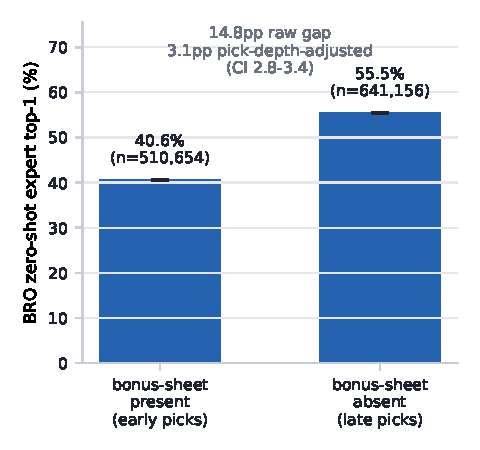
\includegraphics[width=0.55\linewidth]{figures/bro_diagnostics.pdf}
\caption{BRO zero-shot top-1 with high-win-rate players, split by whether
the pack offered at least one of the 63 BRR retro-artifact bonus-sheet
cards (\BonusPresentFrac\% of BRO's picks do). The raw \BonusRawGap pp
gap is mostly a pick-depth confound (labeled above the bars):
\emph{has\_bonus} tracks early-vs-late pick number by construction, and
stratifying by pick number before comparing collapses the gap to
\BonusStratGap pp (95\% CI). Error bars on the raw bars are 95\%
cluster-bootstrap CIs over drafts, computed from cached zero-shot
predictions.}
\label{fig:bro-diagnostics}
\end{figure}

\paragraph{Skill conditioning.}
Conditioning is a scorer-side input (\S\ref{sec:arch}), so one model
serves any audience. In human-model mode (\S\ref{sec:protocol}) the model
scores \FdevBroAllUsers\% / \FdevTmtAllUsers\% /
\FdevSosAllUsers\% on BRO / TMT / SOS: within a point of the
high-win-rate deployment numbers, consistent with skill moving picks
less than card quality does. Whether MSH shows the same pattern is a
question for the frozen pass (\S\ref{sec:msh}).

\begin{figure}[t]
\centering
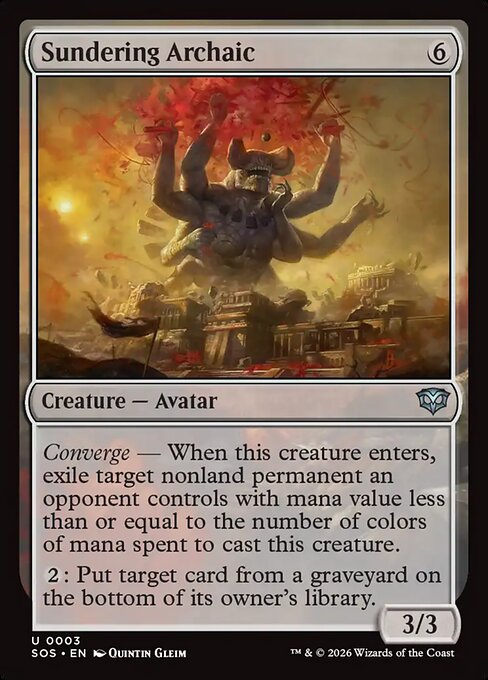
\includegraphics[width=0.12\linewidth]{figures/cards/sundering-archaic.jpg}%
\hspace{2mm}%
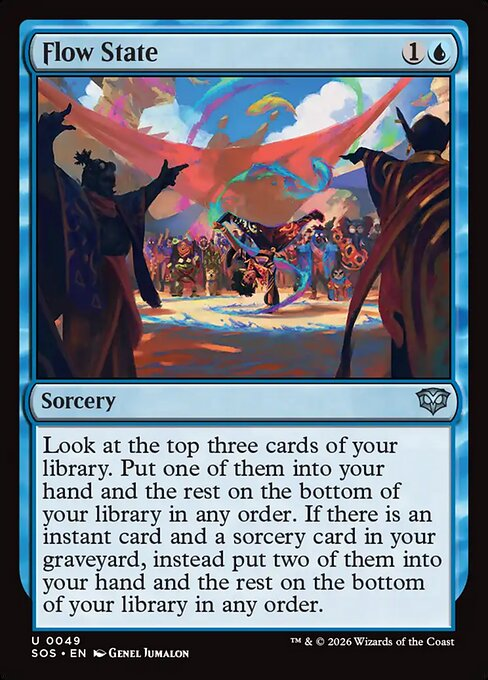
\includegraphics[width=0.12\linewidth]{figures/cards/flow-state.jpg}
\caption{The low-conviction end of the model's output: an illustrative
thirteen-card SOS pack (empty pool) where \VCCNameA{} and \VCCNameB{} score a near-exact
tie (EV \VCCEvA{} vs.\ \VCCEvB, dominance split \VCCSplitA/\VCCSplitB) --
the third candidate, \VCCRunnerName, trails at \VCCRunnerPct\% dominance
against the pair. Ties this close are exactly the regime the top-label ECE
below is measuring: the model's stated confidence and its actual
reliability at low conviction. Computed by the deployed per-set model.}
\label{fig:closecall}
\end{figure}

\paragraph{Calibration.}
% scripts/fit_dev_temperature.py, run=20260704_135822_f_dev. T=1 parity
% check against the published per-set ECE macros passed exactly before
% any T was chosen. Grid 0.30:3.00:0.02; frozen T selected by argmin mean
% dev-trio log-loss (Guo et al. 2017 convention), not ECE directly (ECE-
% argmin lands at T=1.40, mean ECE 0.0133, ~2x lower than the log-loss
% choice's 0.0250 -- so this leaves ECE on the table by design: log-loss is
% the smooth, proper scoring rule this protocol's other dev decisions
% already prefer, chosen over directly optimizing the number quoted in
% the text). Frozen into
% experiments/frozen_battery.json's "calibration" block before T0, applied
% to both deployment and human mode.
Zero-shot confidence falls well short of within-set calibration. Top-label
ECE is \FdevBroEce{} / \FdevTmtEce{} / \FdevSosEce{} on the dev trio,
against \CeilSosEce{} for the within-set SOS reference: roughly a five- to
seven-and-a-half-fold gap. The protocol permits one calibration decision: a
temperature fitted on dev only and frozen into the battery, never fitted
on MSH. That temperature is \FrozenTemperature, chosen by minimizing mean
dev-trio log-loss over a grid rather than ECE directly, since log-loss is
the smooth, proper scoring rule this protocol's other dev decisions
already use. It cuts the dev-trio mean ECE from \DevMeanEceAtTOne{} at the
unscaled T=1 to \DevMeanEceAtFrozenT{}, closing most of the gap above.
This temperature is fit on the logits of F-dev, the architecture-search
model that still has the set-context tower (\S\ref{sec:arch}), and applied
unchanged at test time to F-full, the tower-free recipe that actually
scores MSH. F-full has no held-out set of its own to fit a temperature
against without touching MSH, which is why the temperature crosses
architectures this way. How that crossed-over temperature fares on MSH
itself is reported with the frozen results (\S\ref{sec:msh}).

\paragraph{Late-draft retention.}
% scripts/eval_late_draft_retention.py, run=20260704_135822_f_dev, picks
% pack/pick-indexed >= 7 (0-indexed) vs. the per-set ceiling's own late
% picks. late_draft_retention: BRO 0.8180, TMT 0.8784, SOS 0.8925, dev-mean
% 0.8630 -- all higher than the corresponding overall (all-pick) ratios
% (0.745/0.810/0.805, dev-mean 0.787). Per-(pack,pick) curve: minimum
% margin (zero-shot top1 - random floor) over every non-forced-pick cell
% is 0.205 (BRO), 0.325 (TMT), 0.284 (SOS).
% Confound check (expert-slice zeroshot parquets, same run, computed
% directly from pack_size/target_rank, no new script): forced-pick rate
% (pack_size==1) at late picks vs overall -- BRO 0.1248 vs 0.0665, TMT
% 0.1435 vs 0.0735, SOS 0.1428 vs 0.0714 (roughly 2x). Mean pack_size late
% vs overall -- BRO 4.50 vs 8.01, TMT 3.98 vs 7.30, SOS 4.00 vs 7.50.
% Genuine (non-trivial, pack_size>=4) late top-1 vs overall top-1 -- BRO
% 0.4536 vs 0.4889, TMT 0.5397 vs 0.5750, SOS 0.5609 vs 0.5652: BELOW
% overall on all three, opposite of the raw retention ratio's direction.
Later picks are where a set-agnostic model could plausibly collapse to
rate-the-card, since pool signal has taken over from the card alone. The
pre-registered statistic, late-draft retention (\S\ref{sec:protocol}), is
\LateRetBro\% / \LateRetTmt\% / \LateRetSos\% on BRO / TMT / SOS (dev-mean
\LateRetDevMean\%), higher, not lower, than the corresponding all-pick
ratios (\RatioBro\% / \RatioTmt\% / \RatioSos\%, \S\ref{sec:results}). That
raw ratio is not, on its own, evidence that the pool tower is adding
signal late. Picks 8+ carry roughly twice the forced-pick rate of the
draft as a whole (forced picks score 1.0 by construction on both sides of
the ratio) and a substantially smaller mean pack size (4.0--4.5 cards
vs.\ 7.3--8.0 overall). Restricting to genuine choices, pack size $\geq$
4, excluding the trivial tail, puts late-pick top-1 \emph{below} the
all-pick figure on all three dev sets, the opposite direction from the
retention ratio. The claim the data does support is narrower: the model
does not collapse to chance late in the draft. The per-(pack, pick) curves
against the per-cell random floor show this directly, and
Figure~\ref{fig:pick-curves} in \S\ref{sec:msh} plots them for all four
sets. Excluding forced picks, zero-shot top-1 never comes closer than
20.5 (BRO) / 32.5 (TMT) / 28.4 (SOS) percentage points to chance at any
point in the draft, including its latest picks.


\section*{Acknowledgments}
This work would not exist without \seventeenlands{}, whose public datasets
\citep{seventeenlands} are the training and evaluation corpus, and whose
data-sharing policy makes reproducible drafting research possible. Card
metadata is provided by Scryfall \citep{scryfall}. \mtg{} is the property of
Wizards of the Coast; this is unofficial research, unaffiliated with and
unendorsed by Wizards of the Coast, \seventeenlands{}, or Scryfall.

\bibliographystyle{plainnat}
\bibliography{references}

\appendix
\section{Limitations}
\label{sec:limitations}

\paragraph{The target is agreement, not optimality.}
Top-1 agreement with expert humans measures imitation. Experts disagree
with each other (the within-set ceiling is ${\sim}70\%$, not 100\%), and
agreeing with them is not the same as maximising win rate; a model could
in principle draft better than its agreement suggests, or worse. Win-rate
evaluation of zero-shot drafters is future work.

\paragraph{Population.}
\seventeenlands{} users are self-selected: they run a tracker, they draft
on Arena, and the expert slice further conditions on volume and success.
All numbers are relative to this population; paper drafting, other
platforms, and casual play are out of scope.

\paragraph{One evaluation round.}
Pre-registration buys credibility at the cost of adaptivity: the frozen
battery cannot react to surprises in the test snapshot, and a single set
is a sample of one from the distribution of future sets. The dev-trio
spread and the composition probes bound, but do not eliminate,
set-to-set variance in what the headline number would be on the
\emph{next} set.

\paragraph{Text and language.}
The text encoder is English-only and frozen; rules text is embedded as
prose, so mechanics whose meaning is mostly numeric or positional may be
under-represented. Name masking removes the most direct pretraining
leak for licensed sets, but flavor vocabulary in the remaining text still
differs by universe (\S\ref{sec:analysis}).

\paragraph{Numerics.}
Training runs on an accelerator backend with documented silent-error
classes; we gate on CPU parity and skip non-finite steps
(\S\ref{sec:training}), which guards the classes we know about.

\section{Reproducibility}
\label{sec:repro}

Every training and evaluation run appends one record to an append-only
ledger: run id, git sha, protocol tag, seed, framework version, full
config, data-manifest hash, wall clock, throughput, artifact sha256s, and
dev metrics. Every table cell in this paper carries its source run id as
a comment in the generated table file; tables and the scaling figure are
emitted by a script from run records and cached evaluation outputs, and
the prose reads numbers from generated macros, so no result number in
this document is typed by hand.

Frozen identifiers: protocol tag \texttt{\ProtocolTag}; data-manifest
content hash \texttt{\DataManifestHash}; featurizer-manifest content hash
\texttt{\FeaturizerHash}; F-dev run \texttt{\FdevRunId}. The MSH snapshot
sha256 and ETag are recorded at freeze time and reported here:
\pending{MSH snapshot sha256, ETag, download timestamp, gate report}.

Released with the paper: training and evaluation code, the frozen
protocol document and metric implementations, data and featurizer
manifests, model weights for every battery member, and the per-pick
prediction files from which every statistic is computed (archived on
Zenodo). Raw \seventeenlands{} bytes for the test snapshot are deposited
only after a courtesy note to \seventeenlands{}; all other inputs are
re-derivable from public sources via the manifests.

\section{Licensing and attribution}
\label{sec:licensing}

\paragraph{Draft data.}
Draft data is from the \seventeenlands{} public datasets
\citep{seventeenlands}, used under CC BY 4.0 and per the project's usage
guidelines (bulk S3 downloads; no API scraping).

\paragraph{Card metadata.}
Card metadata is from Scryfall \citep{scryfall}, used per its API
guidelines; Scryfall neither produces nor endorses this work.

\paragraph{Card images.}
Figures~\ref{fig:teaser}, \ref{fig:bro-tierlist}, and \ref{fig:closecall}
reproduce official Scryfall card scans \citep{scryfall}, fetched directly
from Scryfall's own hosted image URLs by
\texttt{figures/fetch\_example\_cards.py} (released with the paper, along
with the cached images and their source manifest). Scryfall's stated
policy on card images (``Use of Scryfall Data and Images,''
\url{https://scryfall.com/docs/api}) permits this use, subject to rules we
follow throughout: every image is shown full and unmodified---no
cropping, distorting, blurring, sharpening, desaturating, color-shifting,
or watermarking of the card art itself---and any score or label in a
figure sits beside the image, never on top of it. Because the full card
image is always used (never an art crop), the copyright and artist line
Scryfall prints at the bottom of the card remains visible in every
figure, and nothing here implies that Wizards of the Coast produced or
endorses this work. The cards illustrated are drawn from BRO and
SOS---public, released development sets (\S\ref{sec:data})---never from
MSH, which remains untouched until the frozen evaluation of
\S\ref{sec:protocol}.

\paragraph{Wizards of the Coast intellectual property.}
Portions of the materials used, including all card names, text, and art
shown in figures, are property of Wizards of the Coast. \copyright{}
Wizards of the Coast LLC. This work contains unofficial Fan Content
permitted under the Wizards of the Coast Fan Content Policy; it is not
approved or endorsed by Wizards of the Coast. \mtg{} and its card names
and text are trademarks and copyrights of Wizards of the Coast.
Licensed-IP card names and imagery appear only as printed on the official
card or as data strings in sourced fields of the released artifacts, and
are the property of their respective rights holders---Marvel's for MSH,
the Teenage Mutant Ninja Turtles franchise's for TMT---distinct
properties, both used by Wizards of the Coast under license and neither
affiliated with this paper.


\end{document}
